\documentclass[12pt]{iopart}

\usepackage{iopams}

\makeatletter
\@namedef{ver@amsmath.sty}{}
\makeatother

\usepackage{siunitx}
\usepackage[colorinlistoftodos,textsize=tiny]{todonotes} % TODO: remove me before submitting
\usepackage{isotope}
\usepackage{fixltx2e}
\usepackage{booktabs}
\usepackage{multirow}
\usepackage{url}
\usepackage{graphicx}

\providecommand{\keywords}[1]{\textbf{\textit{Index terms---}} #1}
\newcommand{\DDO}{D\textsubscript{2}O}

\graphicspath{{./fig/}}

\begin{document}

%%%%%%%%%%%%%%%%%%%%%%%%%%%%%%%%%%%%%%%%%%%%%%%%%%%%%%%%%%%%%%%%%%%%%%%%%%%%%%%
% FRONT MATTER
%%%%%%%%%%%%%%%%%%%%%%%%%%%%%%%%%%%%%%%%%%%%%%%%%%%%%%%%%%%%%%%%%%%%%%%%%%%%%%%

\title[Fast Regression of the Tritium Breeding Ratio in Tokamaks]{Fast Regression of the
Tritium Breeding Ratio in Tokamak Fusion Reactors} % TODO: revise this

\author{G~Van Goffrier$^1$ and P~Mánek$^{1,2}$, V~Gopakumar$^3$, N~Nikolau$^1$, J~Shimwell$^3$, I~Waldmann$^1$}

\address{$^1$ Department of Physics and Astronomy, University College London, Gower Street, London WC1E~6BT, UK}
\address{$^2$ Institute of Experimental and Applied Physics, Czech Technical University, Husova 240/5, Prague 110~00, Czech Republic}
\address{$^3$ UK Atomic Energy Authority, Culham Science Centre, OX14~3DB Abingdon, UK}

\eads{\mailto{graham.vangoffrier.19@ucl.ac.uk}, \mailto{petr.manek.19@ucl.ac.uk}}

\begin{abstract}
	% TODO: this has been taken as is from the report, revise this
	The tritium breeding ratio (TBR) is an essential quantity for the design of
	modern and next-generation Tokamak nuclear fusion reactors. Representing the
	ratio between tritium fuel generated in breeding blankets and fuel consumed
	during reactor runtime, the TBR depends on reactor geometry and material
	properties in a complex manner. In this work, we explored the
	training of surrogate models to produce a cheap but high-quality approximation
	for a Monte Carlo TBR model in use at the UK Atomic Energy Authority. We
	investigated possibilities for dimensional reduction of its feature space, reviewed
	9~families of surrogate models for potential
	applicability, and performed hyperparameter optimisation. Here we present the
	performance and scaling properties of these
	models, the fastest of which, an artificial neural network,
	demonstrated~$R^2=\num{0.985}$ and a mean
	prediction time of~$\SI{0.898}{\micro\second}$, representing a relative speedup of $8\cdot 10^6$
	with respect to the expensive MC model. We further present a novel adaptive
	sampling algorithm, Quality-Adaptive Surrogate Sampling, capable
	of interfacing with any of the individually studied surrogates. Our preliminary
	testing on a toy TBR theory has demonstrated the efficacy of this algorithm for
	accelerating the surrogate modelling process.
\end{abstract}

% TODO: revise these
\keywords{magnetic moment, solar neutrinos, astrophysics}
\submitto{\jpg}
\maketitle


%%%%%%%%%%%%%%%%%%%%%%%%%%%%%%%%%%%%%%%%%%%%%%%%%%%%%%%%%%%%%%%%%%%%%%%%%%%%%%%
% MAIN MATTER
%%%%%%%%%%%%%%%%%%%%%%%%%%%%%%%%%%%%%%%%%%%%%%%%%%%%%%%%%%%%%%%%%%%%%%%%%%%%%%%

\section{Introduction}
\label{sec:introduction}
The analysis of massive datasets has become a necessary component of virtually all technical fields, as well as the social and humanistic sciences, in recent years. Given that rapid improvements in sensing and processing hardware have gone hand in hand with the data explosion, it is unsurprising that software for the generation and interpretation of this data has also attained a new frontier in complexity. In particular, simulation procedures such as Monte Carlo (MC) event generation can perform physics predictions even for theoretical regimes which are not analytically soluble. The bottleneck for such procedures, as is often the case, lies in the computational time and power which they necessitate.

Surrogate models, or metamodels, can resolve this limitation by replacing a resource-expensive procedure with a much cheaper approximation \cite{Sondergaard2003}. They are especially useful in applications where numerous evaluations of an expensive procedure are required over the same or similar domains, e.g. in the parameter optimisation of a theoretical model. The term "metamodel" proves especially meaningful in this case, when the surrogate model approximates a computational process which is itself a model for a (perhaps unknown) physical process \cite{Myers2002}. There exists a spectrum between "physical" surrogates which are constructed with some contextual knowledge in hand, and "empirical" surrogates which are derived purely from the underlying expensive model. 

In this internship project, in coordination with the UK Atomic Energy Authority (UKAEA) and Culham Centre for Fusion Energy (CCFE), we sought to develop a surrogate model for the tritium breeding ratio (TBR) in a Tokamak nuclear fusion reactor. Our expensive model was a MC-based neutronics simulation \cite{JonathanCollab}, itself a spherical approximation of the Joint European Torus (JET) at CCFE, which returns a prediction of the TBR for a given reactor configuration. We took an empirical approach to the construction of this surrogate, and no results described here are explicitly dependent on prior physics knowledge.

For the remainder of Section 1, we will define the TBR and set the context of this work within the goals of the UKAEA and CCFE. In Section 2 we will describe our datasets generated from the expensive model for training and validation purposes, and the dimensionality reduction methods employed to develop our understanding of the parameter domain. In Section 3 we will present our methodologies for the comparison testing of a wide variety of surrogate modelling techniques, as well as a novel adaptive sampling procedure suited to this application. After delivering the results of these approaches in Section 4, we will give our final conclusions and recommendations for further work.

\subsection{Problem Description}
\label{sec:problemdescription}

Nuclear fusion technology relies on the production and containment of an
extremely hot and dense plasma. In this environment, by design similar to that
of a star, hydrogen atoms attain energies sufficient to overcome their usual
electrostatic repulsion and fuse to form helium \cite{Hernandez2018}. Early prototype reactors
made use of the deuterium (\isotope[2]{H}) isotope of hydrogen in order to
achieve fusion under more accessible conditions, but achieved limited success.
The current frontier generation of fusion reactors, such as JET and the
under-construction International Thermonuclear Experimental Reactor (ITER), make
use of tritium (\isotope[3]{H}) fuel for further efficiency gain.
Experimentation at JET dating back to 1997 \cite{Keilhacker1999} has made significant headway in
validating deuterium-tritium (D-T) operations and constraining the technology
which will be employed in ITER in a scaled up form.

However, tritium is much less readily available as a fuel source than deuterium.
While at least one deuterium atom occurs for every 5000 molecules of
naturally-sourced water, and may be easily distilled, tritium is extremely rare
in nature. It may be produced indirectly through irradiation of heavy water
(deuterium oxide) during nuclear fission, but only at very low rates which could
never sustain industrial-scale fusion power.

Instead, modern D-T reactors rely on tritium breeding blankets, specialised
layers of material which partially line the reactor and produce tritium upon
neutron bombardment, e.g. by 
\begin{align}
	\isotope[1][0]{n} + \hspace{3pt} \isotope[6][3]{Li} 
	&\longrightarrow \hspace{3pt} 
	\isotope[3][1]{T} + \hspace{3pt}\isotope[4][2]{He} \\
	\isotope[1][0]{n} + \hspace{3pt} \isotope[7][3]{Li} 
	&\longrightarrow \hspace{3pt} 
	\isotope[3][1]{T} + \hspace{3pt} \isotope[4][2]{He} + \hspace{3pt} \isotope[1][0]{n}
\end{align}
\begin{wrapfigure}{r}{0.45\textwidth}
  \vspace{-20pt}
  \begin{center}
    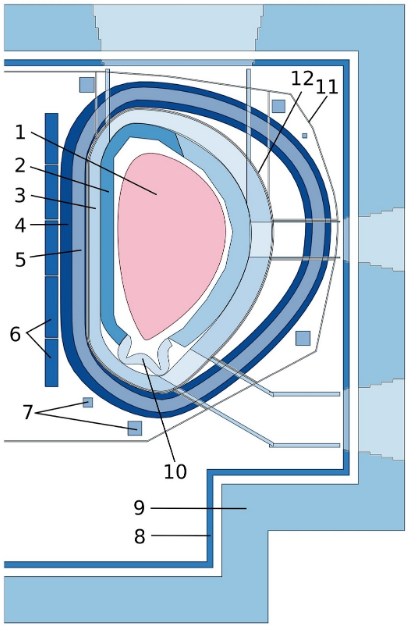
\includegraphics[width=0.48\textwidth]{fig1_tokamakdiagram.png}
  \end{center}
  \caption{Typical single-null reactor configuration as specified by BLUEPRINT \cite{Coleman2019}: 1 — plasma,
2 — breeding blankets }
\label{fig:tokamak}
\end{wrapfigure}
where T represents tritium and \isotope[7]{Li}, \isotope[6]{Li} are the more and
less frequently occurring isotopes of lithium, respectively. \isotope[6]{Li} has
the greatest tritium breeding cross-section of all tested isotopes \cite{Hernandez2018}, but due
to magnetohydrodynamic instability of liquid lithium in the reactor environment,
a variety of solid lithium compounds are preferred.

The TBR is defined as the ratio between tritium generation in the breeding
blanket per unit time and tritium fuel consumption in the reactor. The MC
neutronics simulations previously mentioned therefore must account for both the
internal plasma dynamics of the fusion reactor and the resultant interactions of
neutrons with breeding blanket materials. Neutron paths are traced through a CAD
model (e.g.~\cref{fig:tokamak}) of a reactor with modifiable geometry.

The input parameters of the computationally-expensive TBR model therefore fall
into two classes. Continuous parameters, including material thicknesses and
packing ratios, describe the geometry of a given reactor configuration. Discrete
categorical parameters further specify all relevant material sections, including
coolants, armours, and neutron multipliers. One notable exception is the
enrichment ratio, a continuous parameter denoting the presence of
\isotope[6]{Li}. Our challenge, put simply, was to produce a TBR function which
takes these same input parameters and approximates the MC TBR model with the
greatest achievable accuracy.



\section{Methodology}
\label{sec:methodoglogy}
Assuming that input has been appropriately treated to eliminate redundant
features, we may turn to characterise proposed surrogate models and the criteria
used for their evaluation. The task all presented surrogates strive to solve can be
formulated using the language of conventional regression problems. In the scope
of this work, we explore various possible choices available to us in the
scheme of supervised and unsupervised learning.

Labeling the expensive Monte Carlo simulation $f(x)$, a surrogate is a mapping
$\hat{f}(x)$ that yields similar images as $f(x)$. In other words, $f(x)$ and
$\hat{f}(x)$ minimise a selected similarity metric. Furthermore, in order to
be considered \textit{viable}, surrogates are required to achieve expected evaluation time
that does not exceed the expected evaluation time of $f(x)$.

In the supervised learning setting, we first gather a sufficiently large
training set of samples $\mathcal{T}=\left\{\left( x^{(i)},f\left(x^{(i)}\right) \right)\right\}_{i=1}^N$
to describe the behaviour of $f(x)$ across its domain.
Depending on specific model class and appropriate choice of its
hyperparameters, surrogate models $\hat{f}(x)$ are trained to minimise
empirical risk with respect to $\mathcal{T}$ and a model-specific
loss function $\mathcal{L}$, where empirical risk is defined as

\begin{align}
	R_{\text{emp.}}(\hat{f}\mid\mathcal{T},\mathcal{L})
	=\frac{1}{N}\sum_{i=1}^N
	\mathcal{L}\left(\hat{f}(x^{(i)}),f(x^{(i)})\right).
\end{align}

The unsupervised setting can be viewed as an extension of this method.
Rather than fixing the training set $\mathcal{T}$ for the entire duration of
training, multiple sets $\{\mathcal{T}_k\}_{k=0}^K$ are used, such that
$\mathcal{T}_{k-1}\subset\mathcal{T}_k$ for all $k>1$. The first set
$\mathcal{T}_0$ is initialised randomly to provide a \textit{burn-in}, and is
repeatedly extended in epochs, whereby each epoch trains a new surrogate on
$\mathcal{T}_k$ using the supervised learning procedure, evaluates its
performance, and forms a new set $\mathcal{T}_{k+1}$ by adding more samples to
$\mathcal{T}_k$. This permits the learning algorithm to condition the selection
of new samples by the results of evaluation in order to focus on improvement of
surrogate performance in complex regions within the domain.


\subsection{Metrics}
\label{sec:metrics}

Aiming to provide objective comparison of a diverse set of surrogate model
classes, we define a multitude of metrics to be tracked during experiments.
Following the motivation of this work, two desirable properties of surrogates
arise: (i) their capability to approximate the expensive
model well and (ii) their time of evaluation. An ideal surrogate would maximise
the former while minimising the latter.

\Cref{tbl:metrics} provides exhaustive listing and description of metrics recorded
in the experiments. For regression performance analysis, we include a selection
of absolute metrics to assess the approximation capability of surrogates, and set
practical bounds on the expected accuracy of their predictions. In addition, we also track
relative measures that are better-suited for model comparison between works as
they maintain invariance with respect to the selected domain and image space.
For analysis of evaluation time, surrogates are assessed in terms of wall time
elapsed during training and predicition. This closely models the practical use
case, in which they are trained and used as drop-in replacements for the
expensive model. Since training set sizes remain to be determined, all times are
reported per a single sample. Even though some surrogates support acceleration
by means of parallelisation, measures were taken to ensure sequential
processing of samples to achieve comparability between considered models.

\begin{table}[h]
	\centering
	\begin{tabular}{llrl}
	\toprule
	Regression performance metrics	& Mathematical formulation / description &
	\multicolumn{2}{c}{Ideal value} \\
	\midrule
	Mean absolute error (MAE)	& $\sum_{i=1}^N |y^{(i)}-\hat{y}^{(i)}|/N$ & 0
								& [TBR] \\
	Standard error of regression $S$	& $\text{StdDev}_{i=1}^N\left\{ |y^{(i)} -
	\hat{y}^{(i)}| \right\} $	 & 0 & [TBR] \\
	Coefficient of determination $R^2$	& $1-\sum_{i=1}^N \left(y^{(i)}-\hat{y}^{(i)} \right)^2 /
	\sum_{i=1}^N \left( y^{(i)}-\overline{y} \right)^2 $ & 1 & [rel.] \\
	Adjusted $R^2$	& $1-(1-R^2)(N-1)/(N-P-1)$	& 1 & [rel.] \\
	\midrule
	Evaluation time metrics	& {} & {} & {} \\
	\midrule
	Mean training time $\overline{t}_{\text{trn.}}$	& $(\text{wall training time of
	$\hat{f}(x)$})/N_0$ 	& 0 & [ms] \\
	Mean prediction time $\overline{t}_{\text{pred.}}$	& $(\text{wall prediction time of
	$\hat{f}(x)$})/N$	& 0 & [ms] \\
	Relative speedup	& $(\text{wall evaluation time of $f(x)$}) /
	(N\overline{t}_{\text{pred.}})$	&
	$\to\infty$ & [rel.] \\
	\bottomrule
	\end{tabular}
	\caption{Metrics recorded in supervised learning experiments. In
	formulations, we work with training set of size $N_0$ and testing set of
size $N$, TBR values $y^{(i)}=f(x^{(i)})$ and $\hat{y}^{(i)}=\hat{f}(x^{(i)})$
denote images of the $i$th testing sample in the expensive model and the surrogate
respectively. Furthermore, the mean $\overline{y}=\sum_{i=1}^N y^{(i)}/N$ and $P$ is the
number of input features.}
	\label{tbl:metrics}
\end{table}

To prevent undesirable bias in results due to training set selection, all metrics
collected in the scheme of $k$-fold cross-validation with a standard choice of
$k=5$. Herein, a sample set is subdivided into 5 disjoint folds which are
repeatedly interpreted as training and testing sets, maintaining a constant
ratio of samples between the two. In each such interpretation experiments are
repeated, and the overall value of each metric of interest is reported as the
mean across all folds.


\subsection{Supervised Learning Experiments}
\label{sec:supervised}

\subsubsection{Considered Surrogates}

\begin{table}[h]
	\centering
	\begin{tabular}{llll}
	\toprule
	Surrogate & Acronym & Implementation & Hyperparameters \\
	\midrule
	Support vector machines	& SVM & SciKit Learn & TODO \\
	Gradient boosted trees	& GBT & SciKit Learn & TODO \\
	Extremely random trees	& ERT & SciKit Learn & TODO \\
	AdaBoost	& AB & SciKit Learn & TODO \\
	Gaussian process regression	& GPR & SciKit Learn & TODO \\
	$k$ nearest neighbours	& KNN & SciKit Learn & TODO \\
	Neural networks	& NN & Keras (TensorFlow) & TODO \\
	Inverse distance weighing & IDW & SMT & TODO \\
	Radial basis functions & RBF & SMT & TODO \\
	Stochastic gradient descent & SGD & SciKit Learn & TODO \\
	Ridge regression & RR & SciKit Learn & TODO \\
	Kriging & KRG & SMT & TODO \\
	\bottomrule
	\end{tabular}
	\caption{TODO}
	\label{tbl:surrogates}
\end{table}

TODO: describe classes of surrogates

TODO: reference implementations and original papers

TODO: define NN architectures


\subsubsection{Experiments}

TODO: single slice hyperparameter optimisation

TODO: multislice (mixed) hyperparameter optimisation

TODO: retraining for scaling benchmark

TODO: retraining on large set

\subsection{Adaptive Sampling}
\label{sec:adaptive}



\section{Results}
\label{sec:results}
Having outlined a variety of models and metrics tracked for the
purposes of their objective comparison, we proceed to present and discuss our
results in the next sections.


\subsection{Results of Decoupled Sampling}
\label{sec:modelres}

We begin by comparing a diverse set of surrogate families that we proposed
to evaluate on previously collected samples of the expensive MC TBR model.
Through the four experimental cases described
in~\cref{sec:experiment-methodology}, we aim to study properties of the
considered models in terms of regression performance, training and prediction
time.

\subsubsection{Hyperparameter Tuning}

The first two experiments perform Bayesian optimisation to maximise~$R^2$ in
a cross-validation setting as a function of model hyperparameters. While in the
first experiment we limit training and test sets to the scope of four selected
slices of the feature space, in the second experiment we lift this restriction.

The results displayed in~\cref{fig:exp1-time-vs-reg} indicate that in the first
experiment, GBTs clearly appear to be the most accurate as
well as the fastest surrogate family in terms of mean prediction time. Following
that, we note that ERTs, SVMs and ANNs also achieved satisfactory results with respect to both examined metrics.
While the remainder of tested surrogate families does not exhibit problems in
complexity, its regression performance falls below average.

\begin{figure}[h]
	\centering
	\begin{subfigure}[b]{0.333\textwidth}
		\centering
		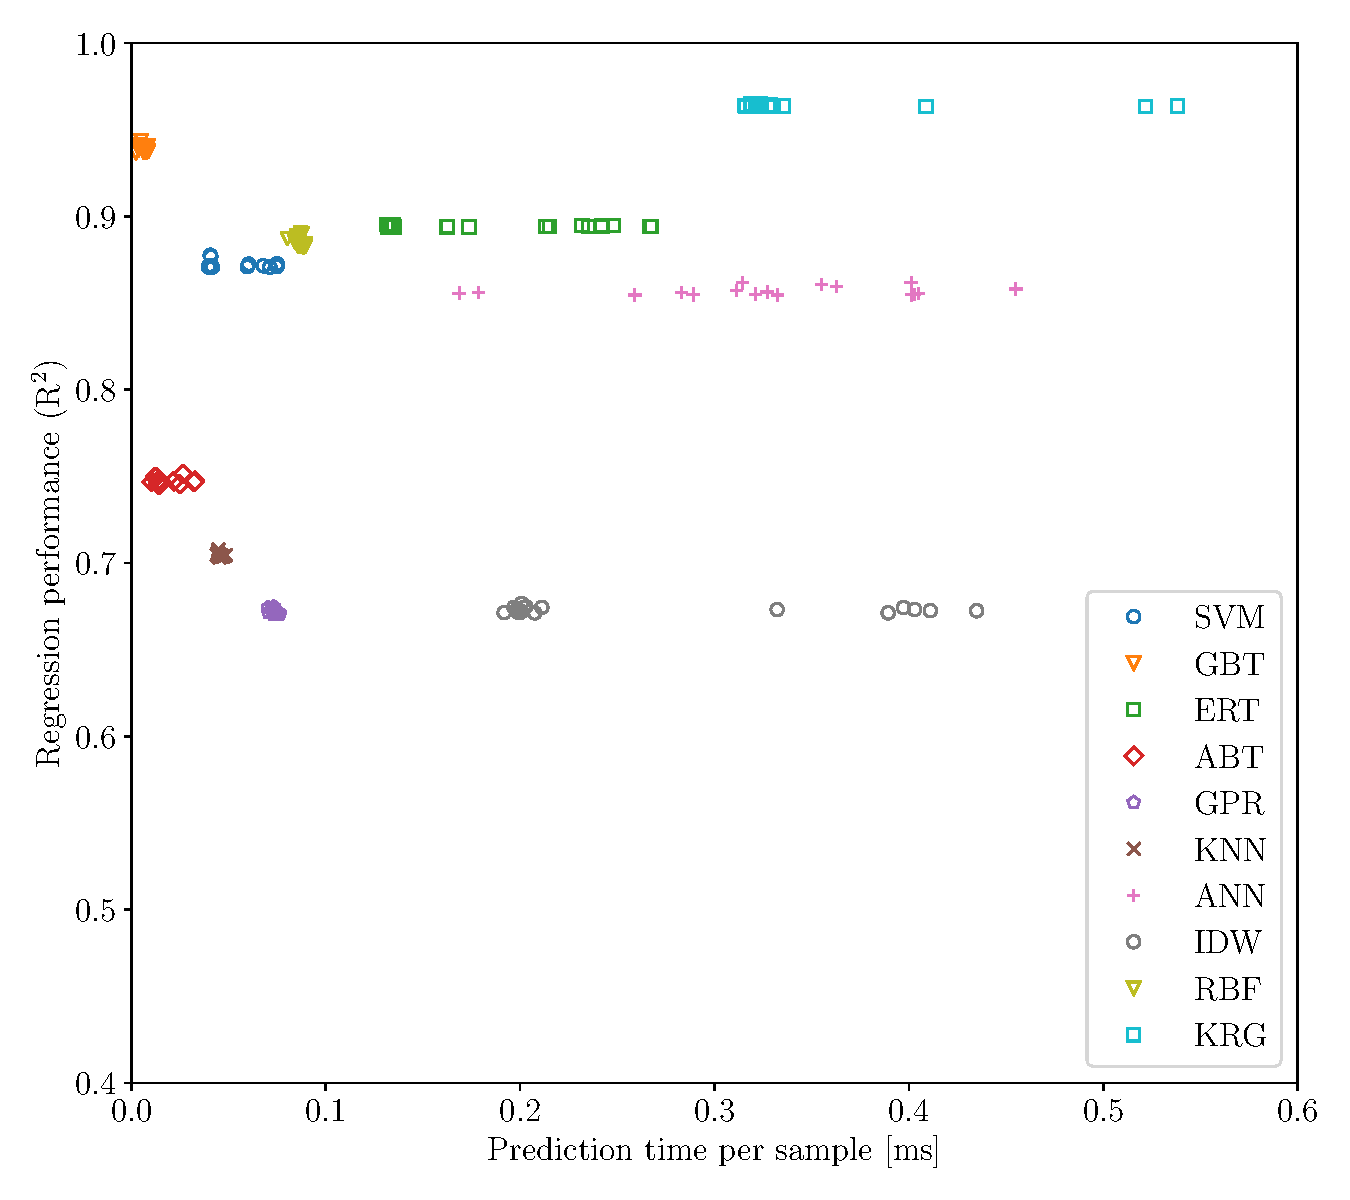
\includegraphics[width=\linewidth]{exp1_slice0}
		\caption{Run 2, batches 0-2}
	\end{subfigure}\hfill%
	\begin{subfigure}[b]{0.333\textwidth}
		\centering
		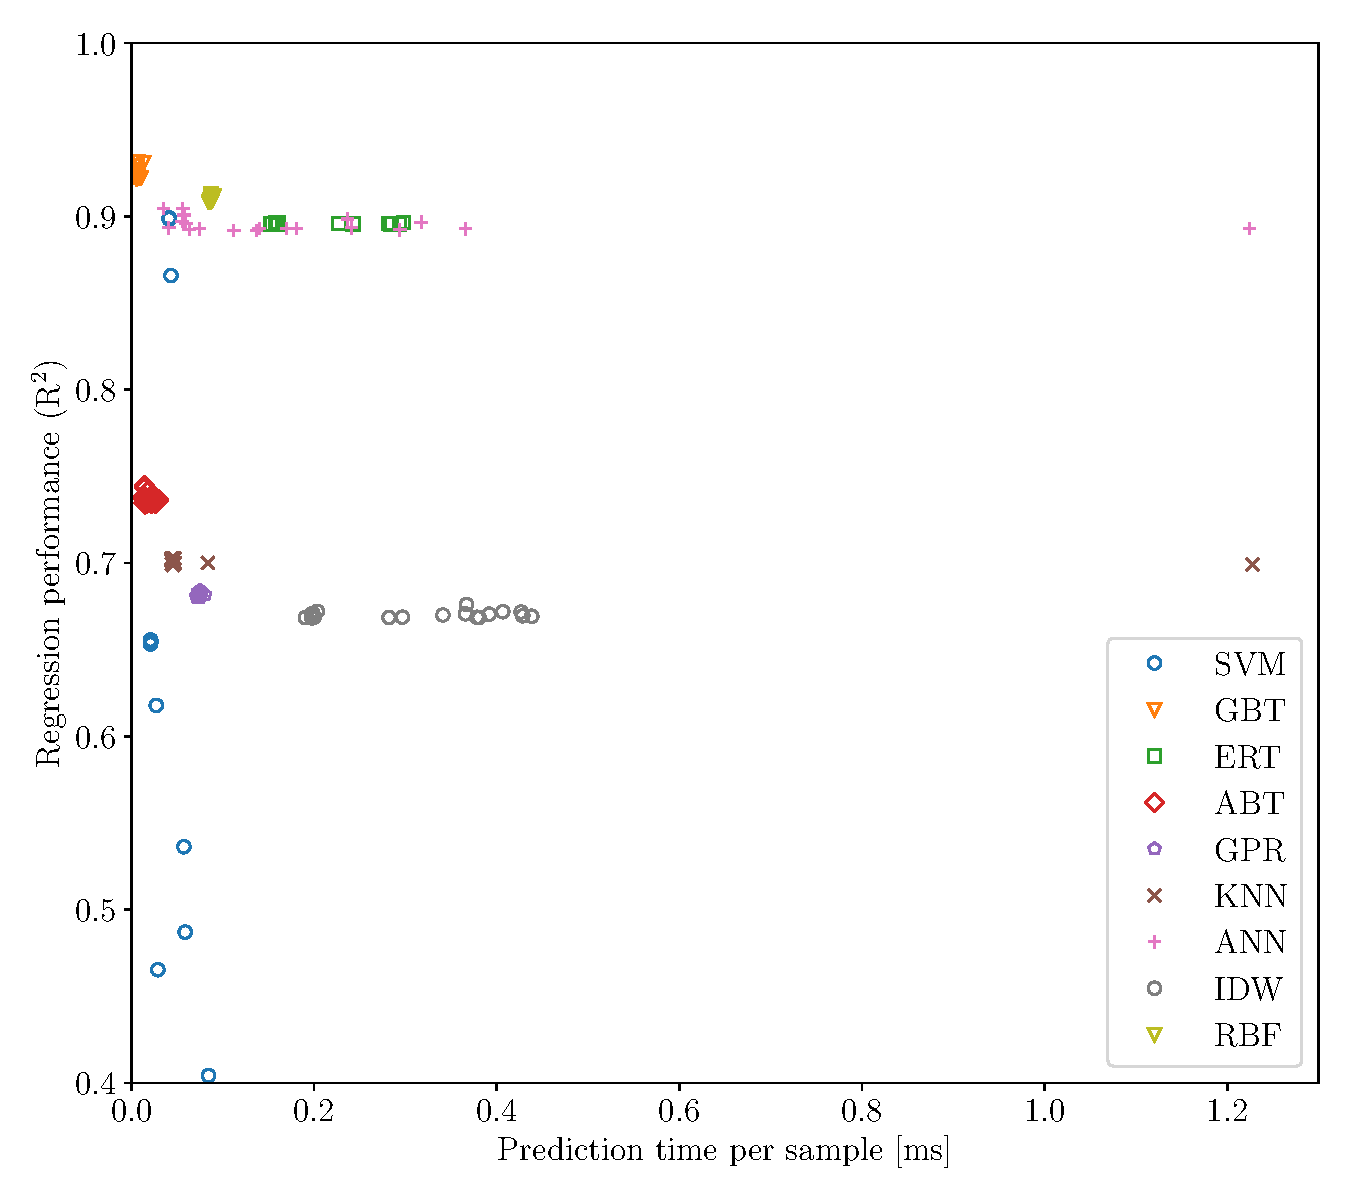
\includegraphics[width=\linewidth]{exp1_slice1}
		\caption{Run 2, batches 100-102}
	\end{subfigure}\hfill%
	\begin{subfigure}[b]{0.333\textwidth}
		\centering
		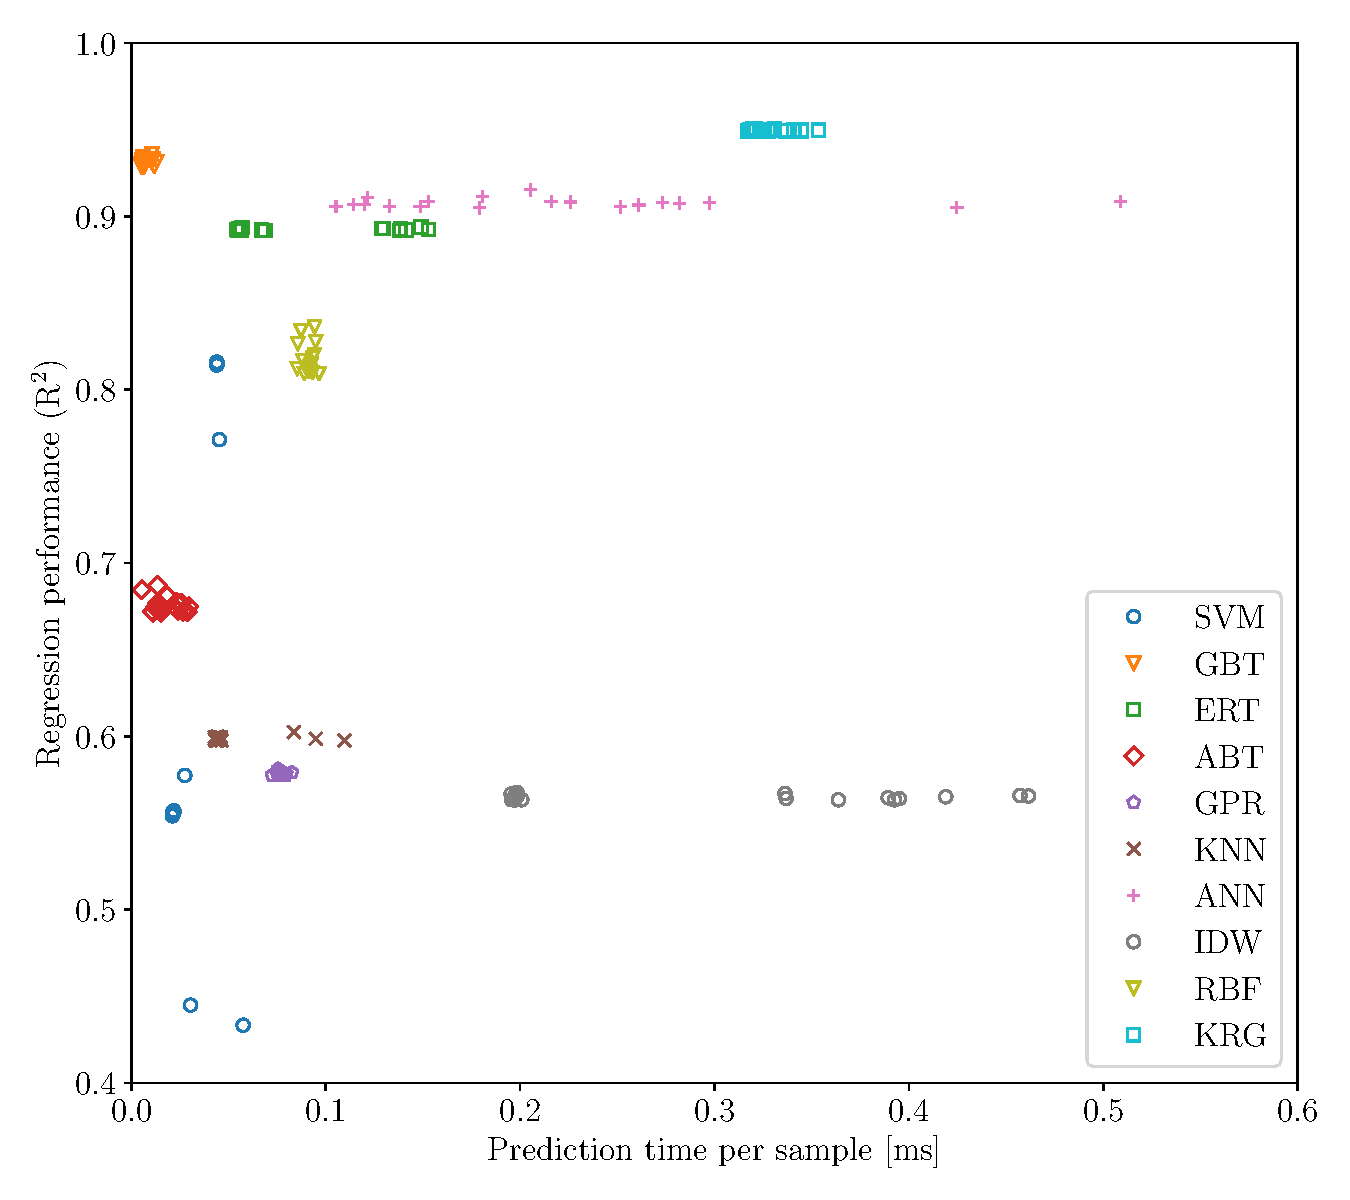
\includegraphics[width=\linewidth]{exp1_slice2}
		\caption{Run 2, batches 200-202}
	\end{subfigure}
	\caption{20~best-performing surrogates per each considered family, plotted in
		terms of complexity (as $\overline{t}_{\text{pred.}}$) and regression
		performance (as~$R^2$) on selected slices of run~2, evaluated in
	experiment~1. Here, batches refer to subsets of training and test datasets that
	may be matched to slices using~\cref{tbl:slices}.}
	\label{fig:exp1-time-vs-reg}
\end{figure}

The results of the second experiment, shown in~\cref{fig:exp2-time-vs-reg},
seem to confirm our expectations. Compared to the previous case, we observe
that many surrogate families consistently achieved worse regression
performance and prediction times in a more complex, unrestricted domain. The least
affected models appear to be GBTs, ANNs and ERTs, which are known to be capable of capturing relationships
involving mixed feature types that were deliberately withheld in the first
experiment. With only negligible differences, the first two of these families
appear to be tied for the best performance as well as the shortest prediction
time. We observe that ERTs trees and RBFs also
demonstrated satisfactory results, outperforming the remaining surrogates in
terms of regression performance, and in some cases also in prediction time.

\begin{wrapfigure}[10]{r}{0.333\textwidth}
	\centering
	\vspace{-2ex}
	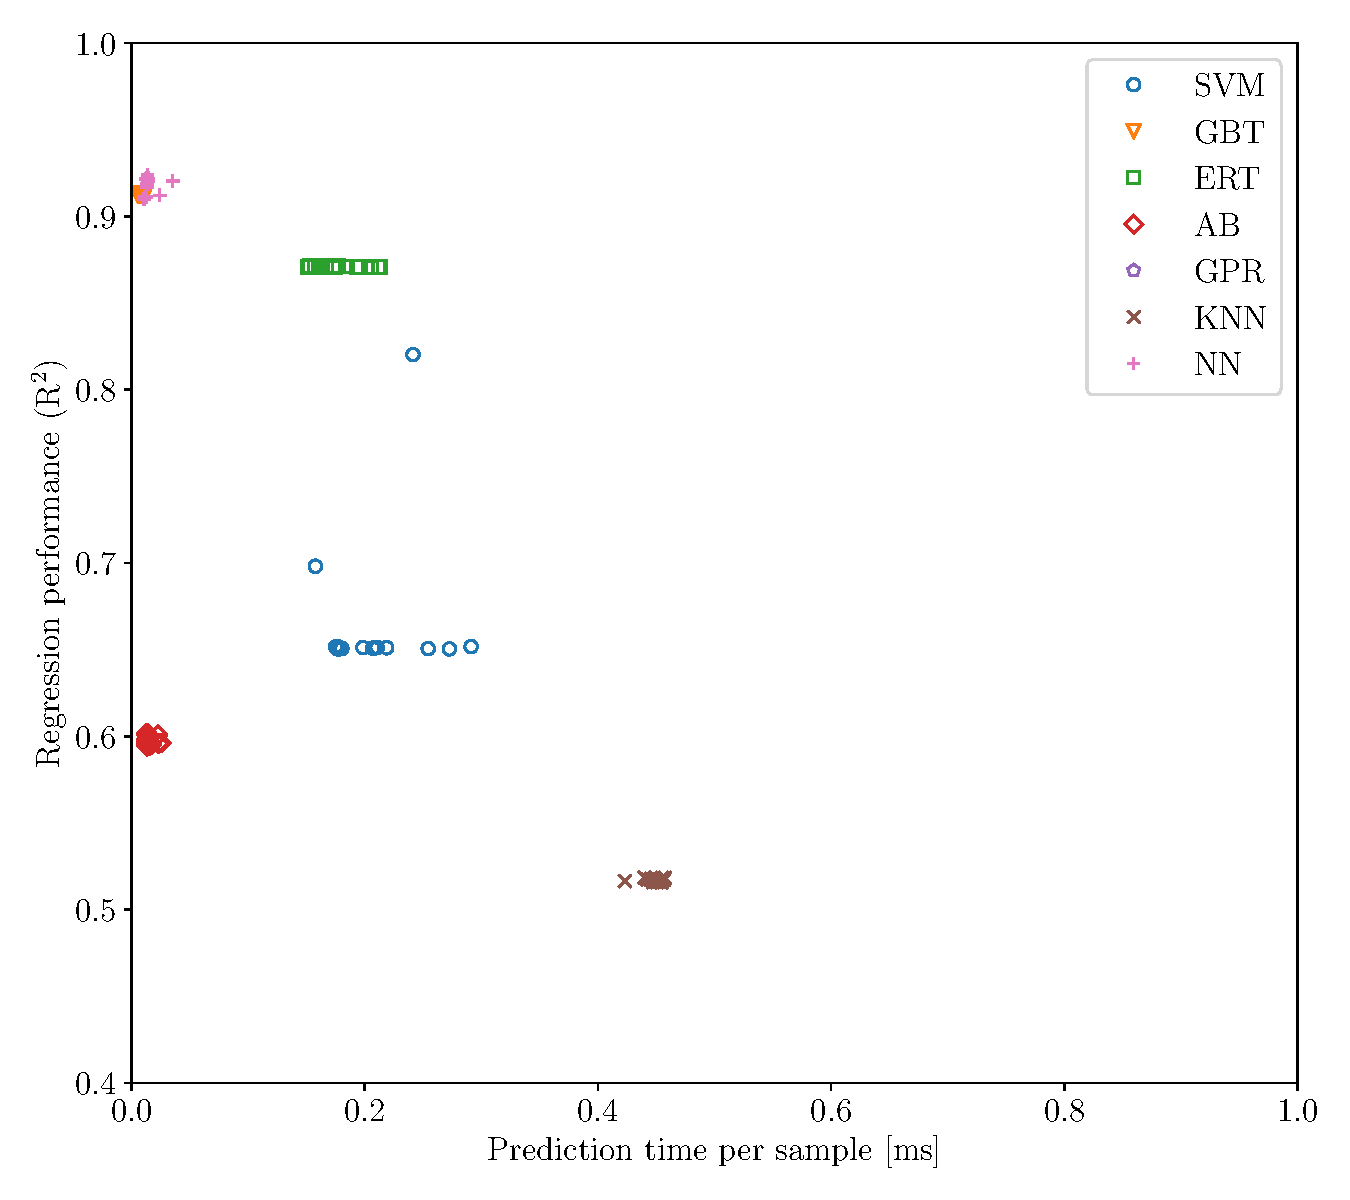
\includegraphics[width=\linewidth]{exp2_time_vs_reg}
	\caption{Results of experiment~2, plotted analogously
	to~\cref{fig:exp1-time-vs-reg}.}
	\label{fig:exp2-time-vs-reg}
\end{wrapfigure}

Following both hyperparameter tuning experiments, we conclude that while domain
restrictions employed in the first case have proven effective in improving the
regression performance of some methods, this result has fluctuated considerably
depending on the selected slices. Furthermore, in all instances the best
results were achieved by families of surrogates that were nearly unaffected by
this modification.


\subsubsection{Scaling Benchmark}

In the third experiment we examine surrogate scaling properties by correlating
metrics of interest with training set size. First, the results shown 
in~\cref{fig:scaling-r2} suggest that the most accurate families from the previous experiments
consistently maintain their relative advantage over others, even as we introduce
more training data. While such families achieve nearly comparable regression
performance on the largest dataset, in the opposite case methods based on
decision trees clearly outperform neural networks. This can be observed
particularly on training sets of sizes up to~\num{6000}.

\begin{figure}[h]
	\centering
	\begin{subfigure}[b]{0.333\textwidth}
		\centering
		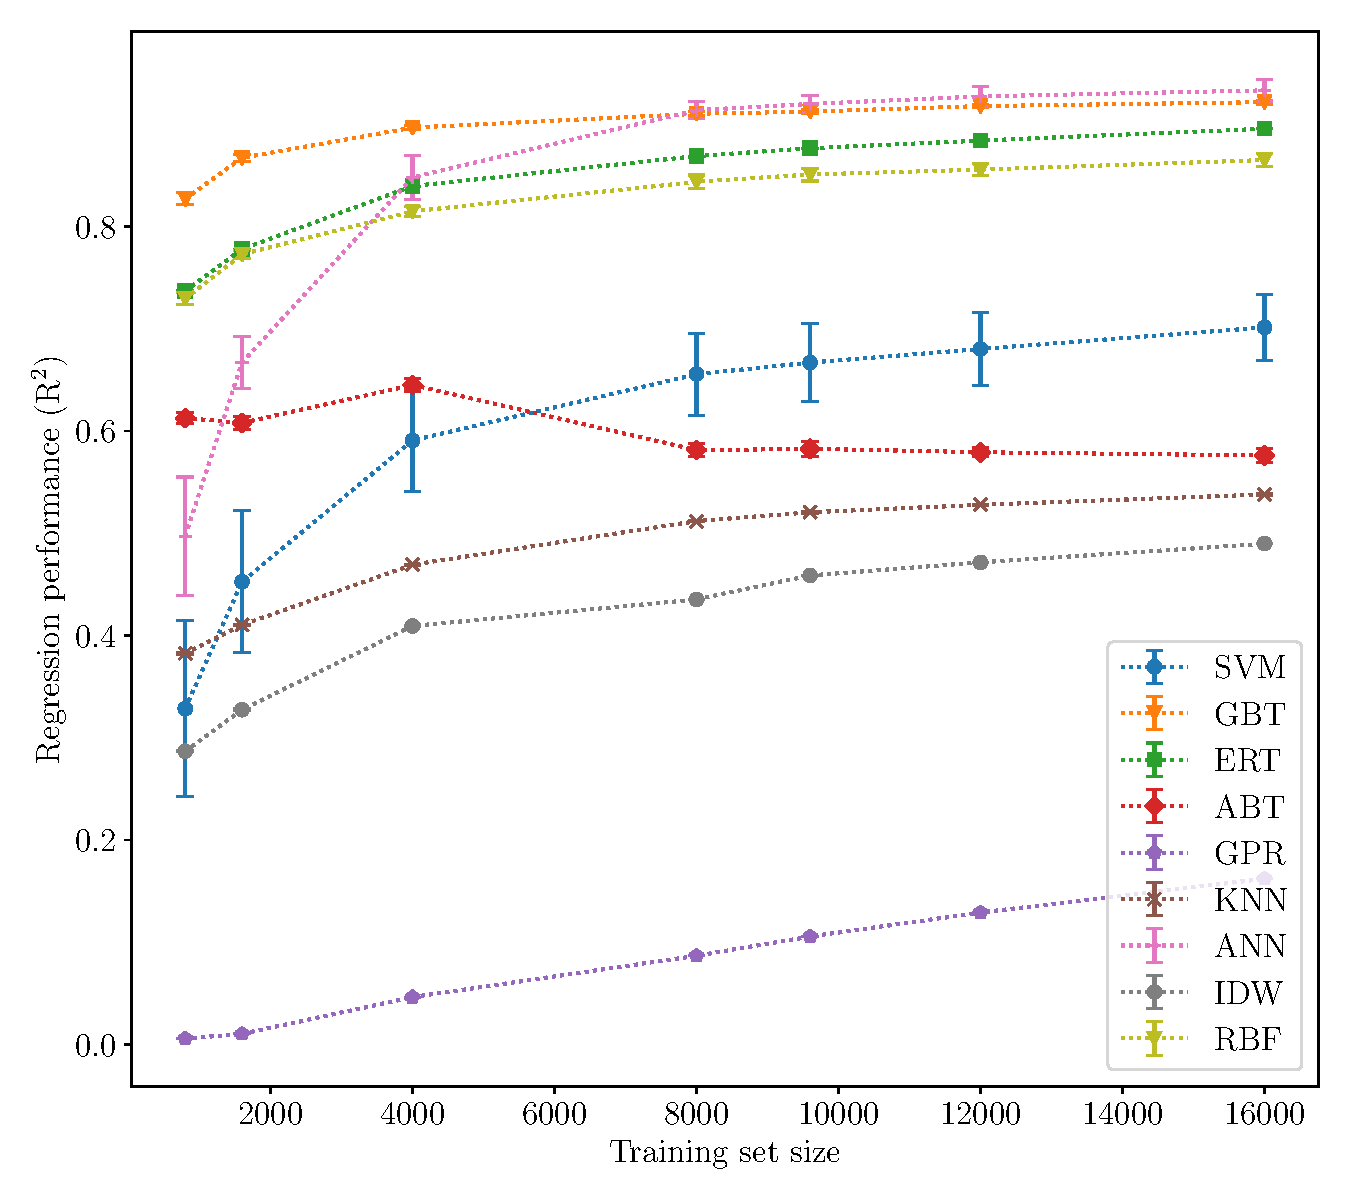
\includegraphics[width=\linewidth]{scaling_metric_r2}
		\caption{Regression performance (as $R^2$)}
		\label{fig:scaling-r2}
	\end{subfigure}\hfill%
	\begin{subfigure}[b]{0.333\textwidth}
		\centering
		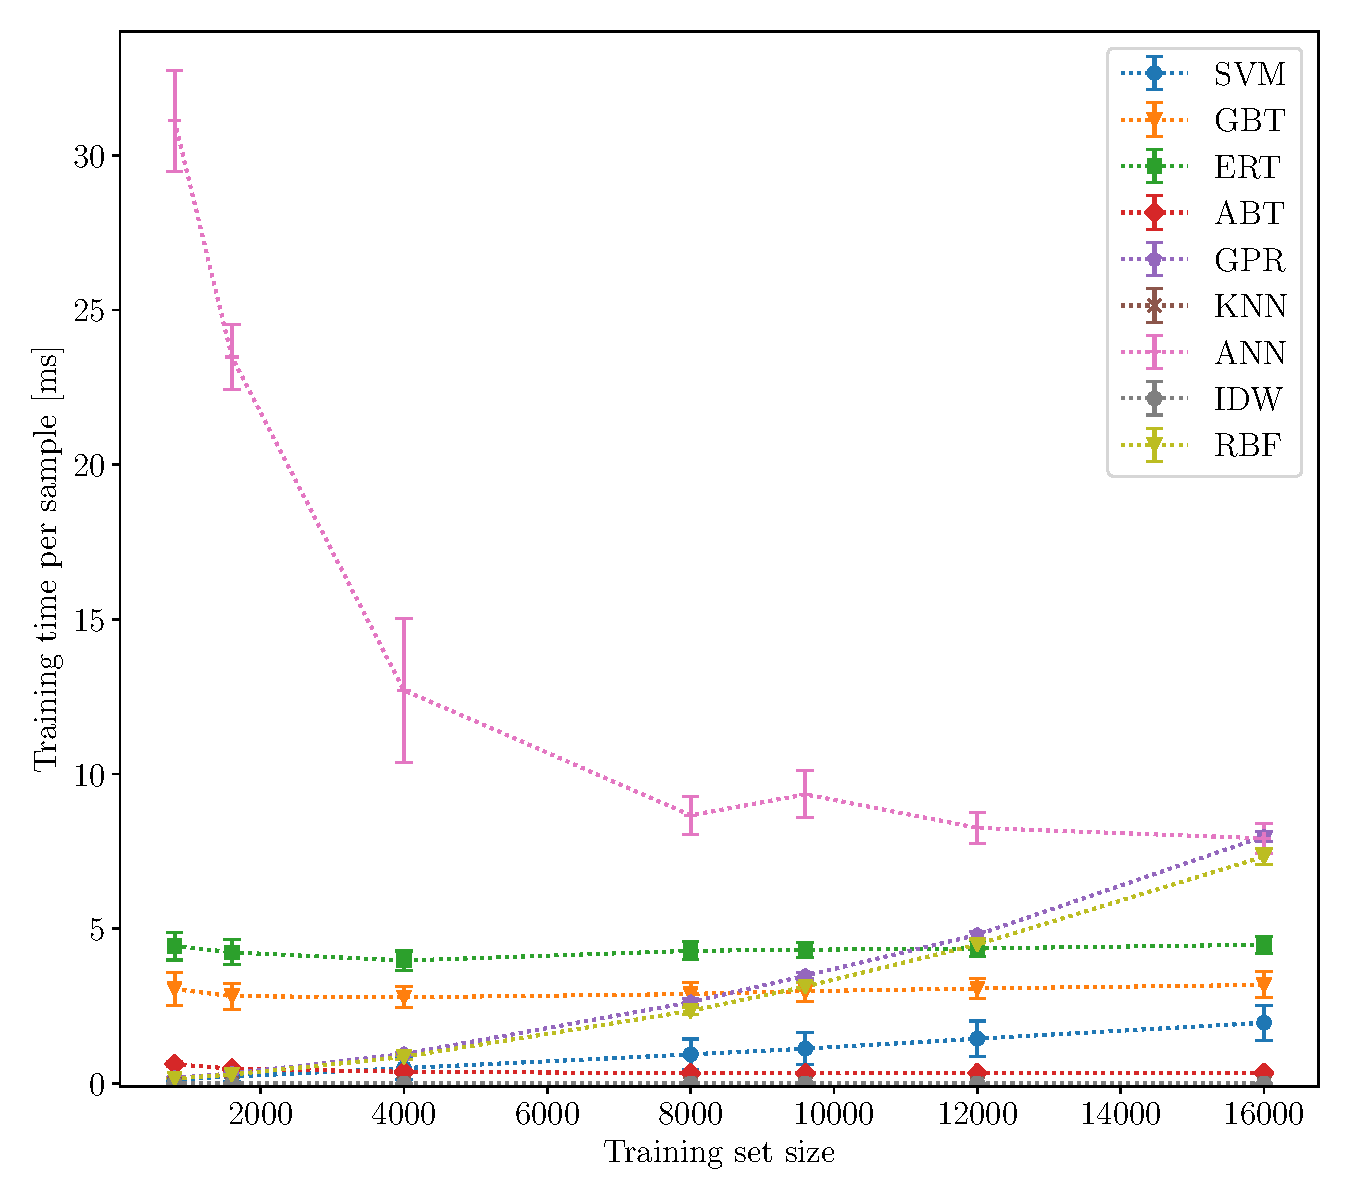
\includegraphics[width=\linewidth]{scaling_time_train}
		\caption{Complexity (as~$\overline{t}_{\text{trn.}}$)}
		\label{fig:scaling-trn}
	\end{subfigure}\hfill%
	\begin{subfigure}[b]{0.333\textwidth}
		\centering
		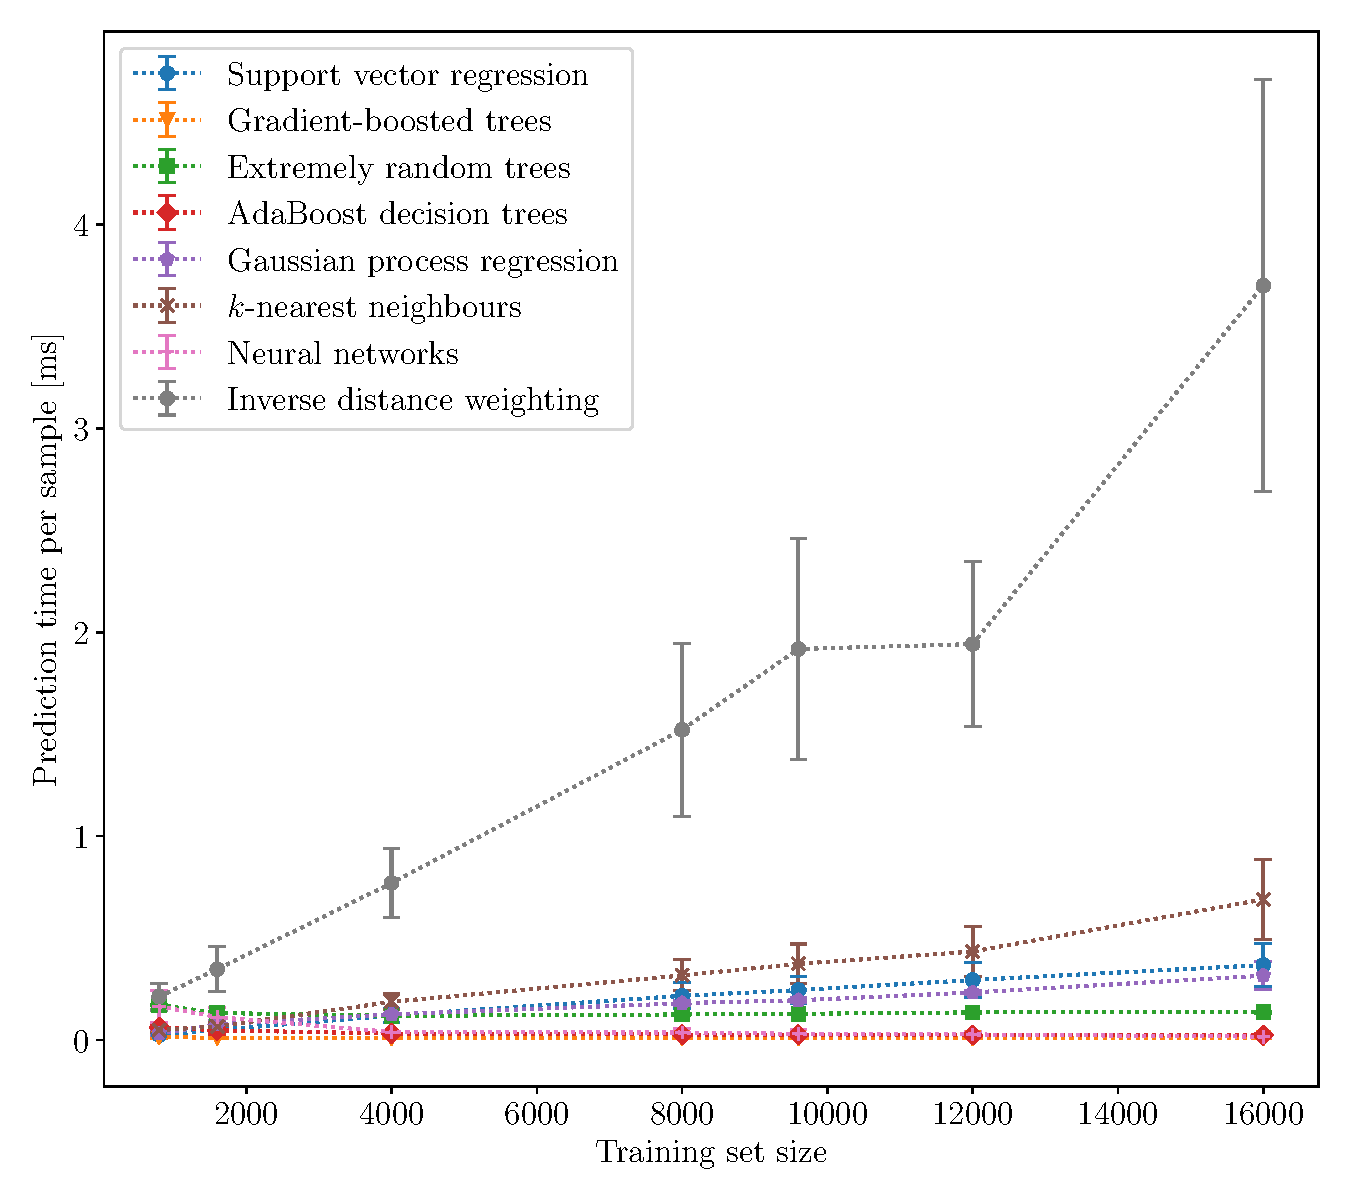
\includegraphics[width=\linewidth]{scaling_time_pred}
		\caption{Complexity (as~$\overline{t}_{\text{pred.}}$)}
		\label{fig:scaling-pred}
	\end{subfigure}
	\caption{Various metrics collected during experiment 3 (scaling
	benchmark) displayed as a function of training set size.}
	\label{fig:scaling}
\end{figure}

Next, we examine scaling behaviour in terms of the mean training time (displayed
in~\cref{fig:scaling-trn}). Consistent with our expectation, the shortest times
were achieved by instance-based learning methods (e.g. KNN, IDW) that
are trained trivially at the expense of increased lookup complexity later during prediction.
Furthermore, we observe that the majority of tree-based algorithms also exhibit
desirable properties unlike RBFs and gaussian process
regression, which appear to scale superlinearly. We note that ANNs,
which are the only family to utilise parallelisation during training, show an
inverse scaling characteristic. Our conjecture is that this effect may be caused
by a constant multi-threading overhead that possibly dominates the training process
on relatively small training sets.

Lastly, we study scaling with respect to the mean prediction time (shown
in~\cref{fig:scaling-pred}). Our initial observation is that all tested
surrogate families with the exception of previously mentioned instance-based
learning methods offer desirable characteristics overall. Analogous to previous
experiments, GBTs and ANNs again
appear to be tied, as they not only exhibit comparable times but also similar
scaling slopes.


\subsubsection{Model Comparison}

In the fourth and final experiment, we exploit previously collected information
to produce surrogates with desirable properties for practical use. We
aim to create models that yield: (i)~the best regression performance regardless
of other features, (ii)~acceptable performance with the shortest mean
prediction time, or (iii)~acceptable performance with the smallest training set.
To this end, we trained 8~surrogates that are presented in~\cref{fig:reg-performance}
(more details are given in~\cref{tbl:exp4-detailed-results} in the Appendix).

\begin{figure}[h]
	\centering
	\begin{subfigure}[b]{0.25\textwidth}
		\centering
		\includegraphics[width=\linewidth]{exp4_model1}
	\end{subfigure}\hfill%
	\begin{subfigure}[b]{0.25\textwidth}
		\centering
		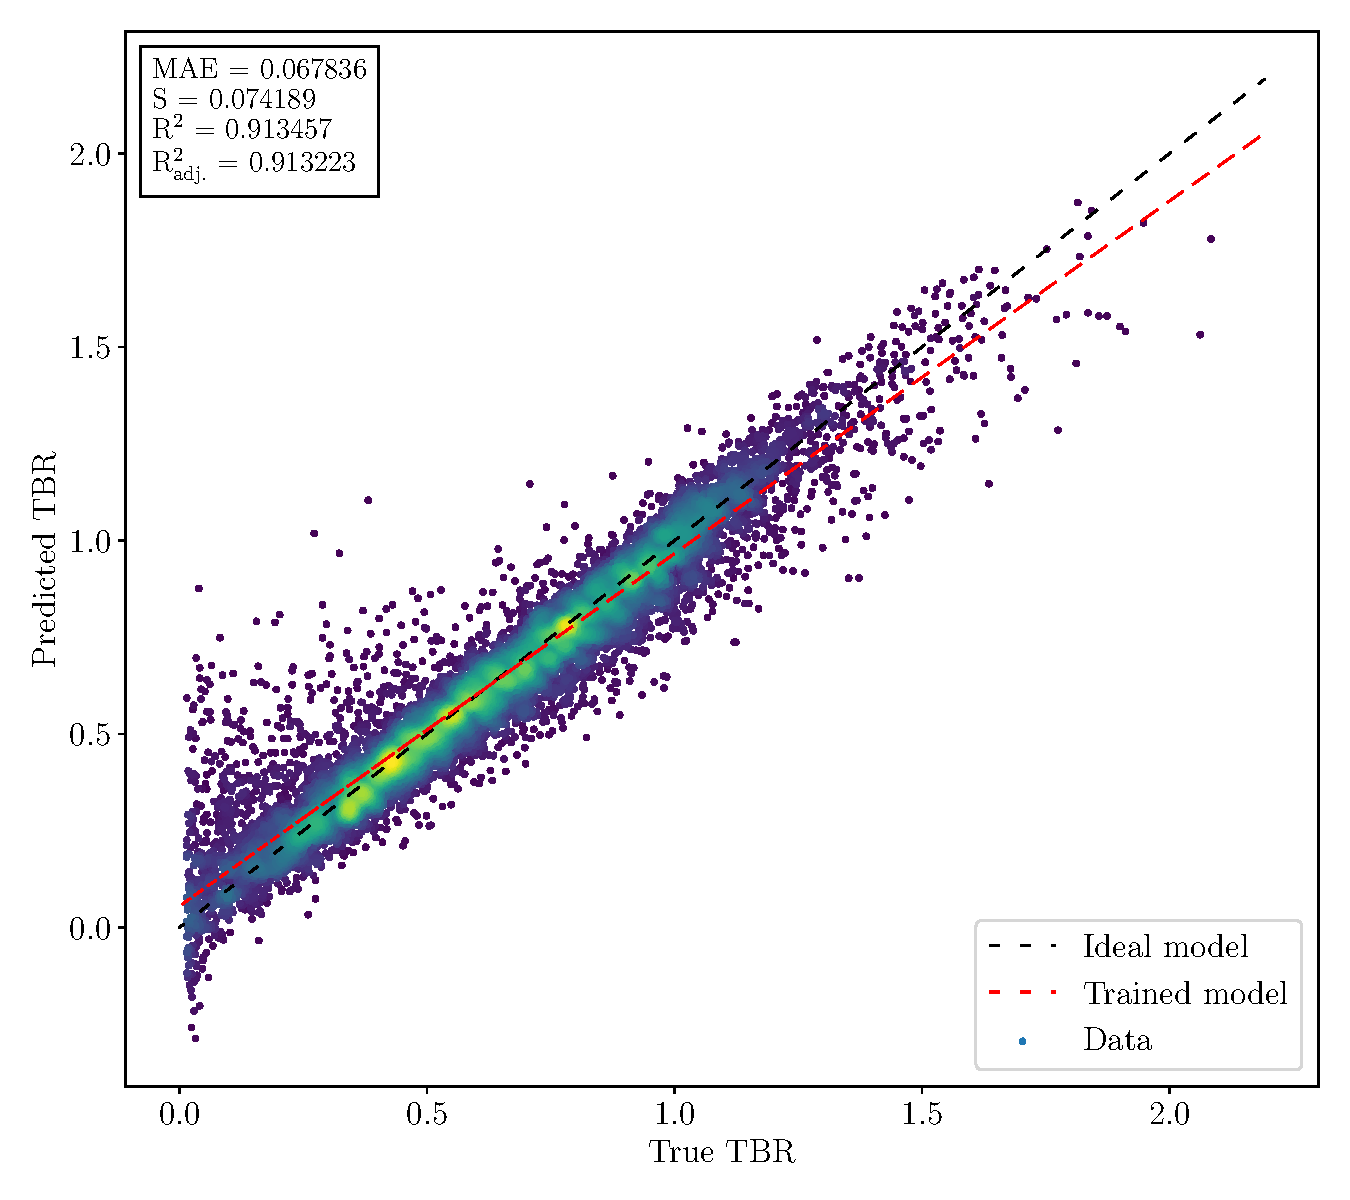
\includegraphics[width=\linewidth]{exp4_model2}
	\end{subfigure}\hfill%
	\begin{subfigure}[b]{0.25\textwidth}
		\centering
		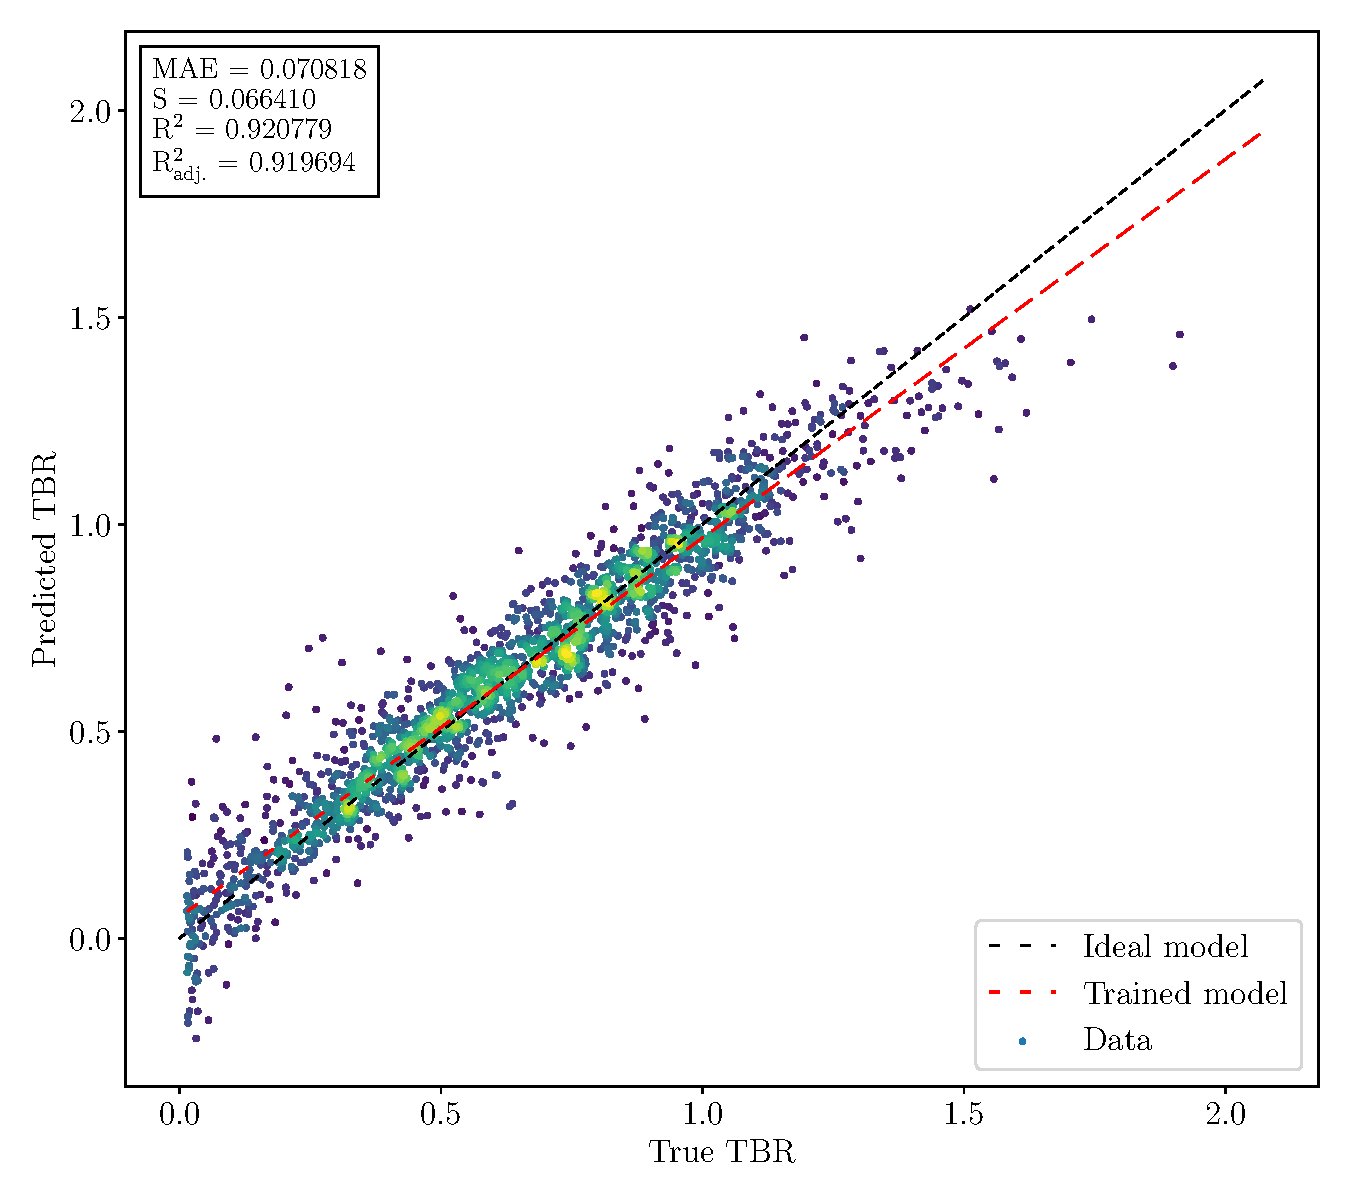
\includegraphics[width=\linewidth]{exp4_model3}
	\end{subfigure}\hfill%
	\begin{subfigure}[b]{0.25\textwidth}
		\centering
		\includegraphics[width=\linewidth]{exp4_model4}
	\end{subfigure}

	\begin{subfigure}[b]{0.25\textwidth}
		\centering
		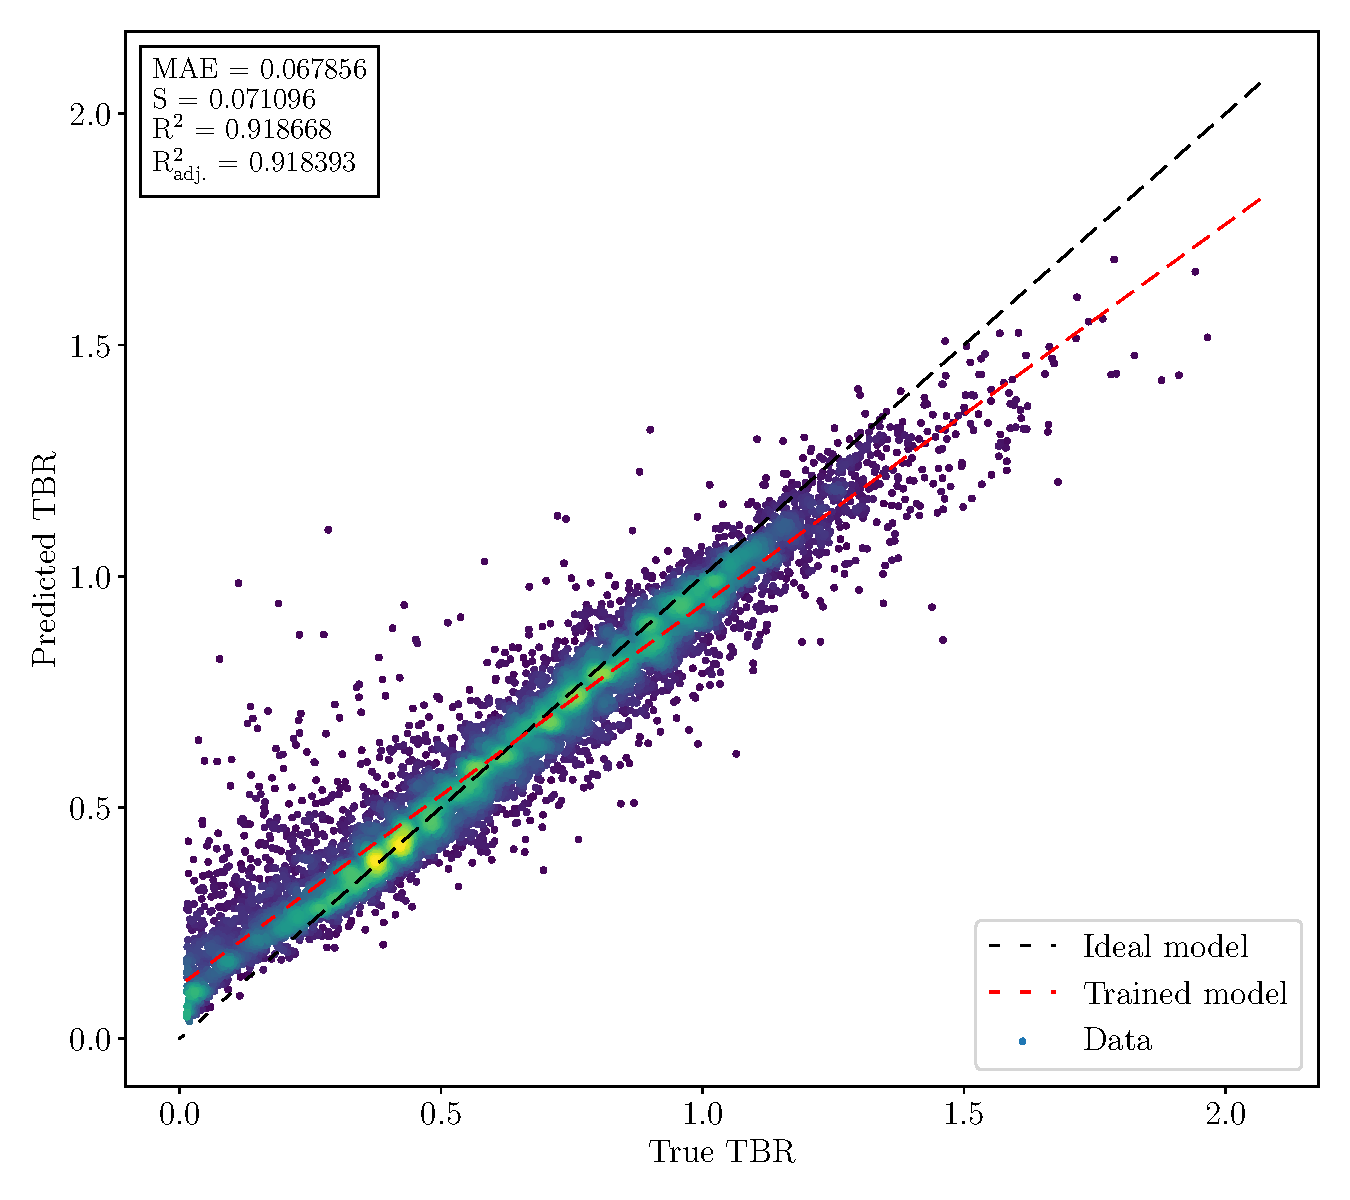
\includegraphics[width=\linewidth]{exp4_model5}
	\end{subfigure}\hfill%
	\begin{subfigure}[b]{0.25\textwidth}
		\centering
		\includegraphics[width=\linewidth]{exp4_model6}
	\end{subfigure}\hfill%
	\begin{subfigure}[b]{0.25\textwidth}
		\centering
		\includegraphics[width=\linewidth]{exp4_model7}
	\end{subfigure}\hfill%
	\begin{subfigure}[b]{0.25\textwidth}
		\centering
		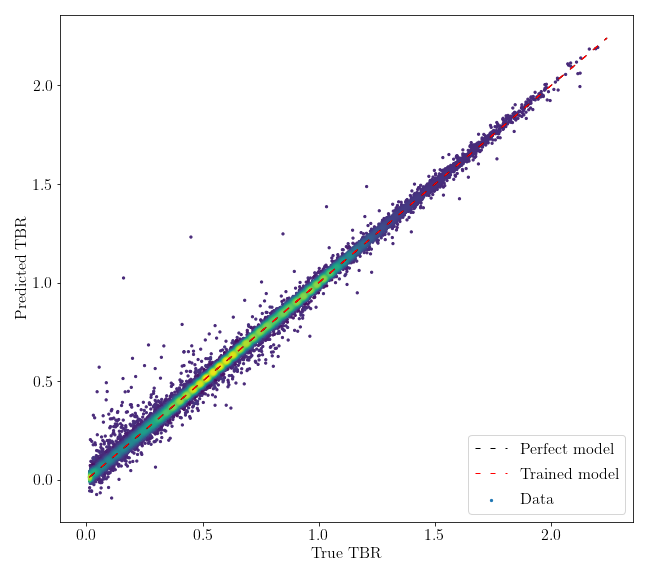
\includegraphics[width=\linewidth]{run1_5ke_1h3f128_4974_performance}
		% TODO: only a placeholder, regenerate when data becomes available
	\end{subfigure}
	\caption{Regression performance of models 1-4 (row 1, from the left) and 5-8
		(row 2) trained in experiment~4 (model comparison), viewed
		as true vs. predicted TBR on a test set of a selected cross-validation
		fold. Points are coloured by density.}
	\label{fig:reg-performance}
\end{figure}

Having selected ANNs, GBTs, ERTs, RBFs and SVMs based on the results of the
experiments~2-3, we utilised the best-performing hyperparameter
assignments and training sets of varying sizes. In attempts to satisfy
goals~(i) and~(ii) within cross-validation setting, our best surrogate
achieved~$R^2=\num{0.998}$ and mean prediction
time~$\overline{t}_{\text{pred.}}=\SI{0.898}{\micro\second}$. These correspond
to the standard error of regression~$S=\num{0.013}$ and a relative speedup~$\omega=\num{8659251} \times$
with respect to the MC TBR evaluation baseline measured during run~1
(see~\cref{tbl:sampling-runs} for details). While this particular surrogate
was trained on the entire available set of~\num{500000} datapoints, in attempts to satisfy
goal~(iii) we also trained a more simplified model that achieved~$R^2=\num{0.913}$,
$\overline{t}_{\text{pred.}}=\SI{6}{\micro\second}$, $S=\num{0.072}$ and $\omega=\num{1269777} \times$
with only a set of size~\num{10000}.

Overall we found that due to their excellent performance, boosted tree-based
approaches seem to be advantageous for fast surrogate modelling on relatively small training
sets (up to the order of~$10^4$). Conversely, while neural networks perform
poorly in such a setting, both their regression performance and prediction times
have proven superior on larger training sets (at least of the order of~$10^5$).


\begin{wrapfigure}[13]{r}{0.4\textwidth}
	\centering
	\vspace{-12ex}
	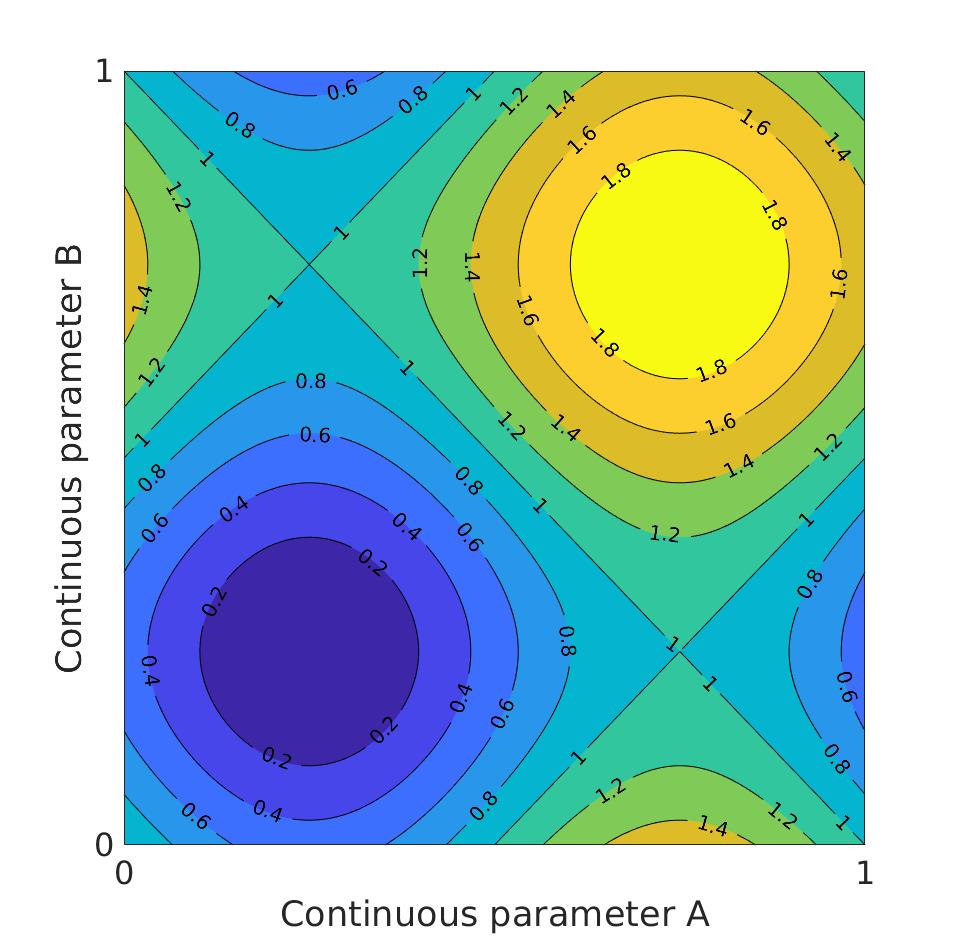
\includegraphics[width=0.4\textwidth]{fig5_sintoy.jpg}
	\caption{Sinusoidal toy TBR theory over two continuous parameters, wavenumber 1}
	\label{fig:sintoy}
\end{wrapfigure}

\subsection{Results of Adaptive Sampling}
\label{sec:adaptiveres}

In order to test our QASS prototype, several functional toy theories for TBR were developed as alternatives to the expensive MC model. By far the most robust of these was the following sinusoidal theory with adjustable wavenumber parameter $n$:

\begin{equation}
	\text{TBR} = \text{Mean}_{i \in C} \left[ \frac{1 + \sin(2\pi n (x_i - 1/2)) }{2} \right]
\end{equation}

plotted in~\cref{fig:sintoy} for $n=1$ and two continuous parameters $C$. ANNs
trained on this model demonstrated similar performance to those on the expensive
MC model. QASS performance was verified by training a $\text{1h3f}(256)$ ANN on
the sinusoidal theory for varied quantities of initial, incremental, and MCMC
candidate samples. Although the scope of this project did not include thorough
searches of this hyperparameter domain, sufficient runs were made to identify
some likely trends.

An increase in MCMC candidate samples was seen to have a positive but very weak
effect on final surrogate precision, suggesting that the runtime of MCMC on each
iteration can be limited for increased efficiency. -- Awaiting test results on
initial sample quantity --. The most complex dynamics arose with the adjustment
of sample increment, shown in~\cref{fig:qassincr}. For each tested initial sample quantity N, the optimal number of step samples was seen to be well-approximated by $\sqrt{N}$; the plotted error trends suggest that incremental samples larger than this optimum give slower model improvement on both the training and evaluation sets, and a larger minimum error on the evaluation set. This performance distinction is predicted to be even more significant when trained on the expensive MC model, where the number of sample evaluations will serve as the primary bottleneck for computation time.
\begin{figure}[h!]
    \centering
    \begin{subfigure}[t]{0.5\textwidth}
        \centering
        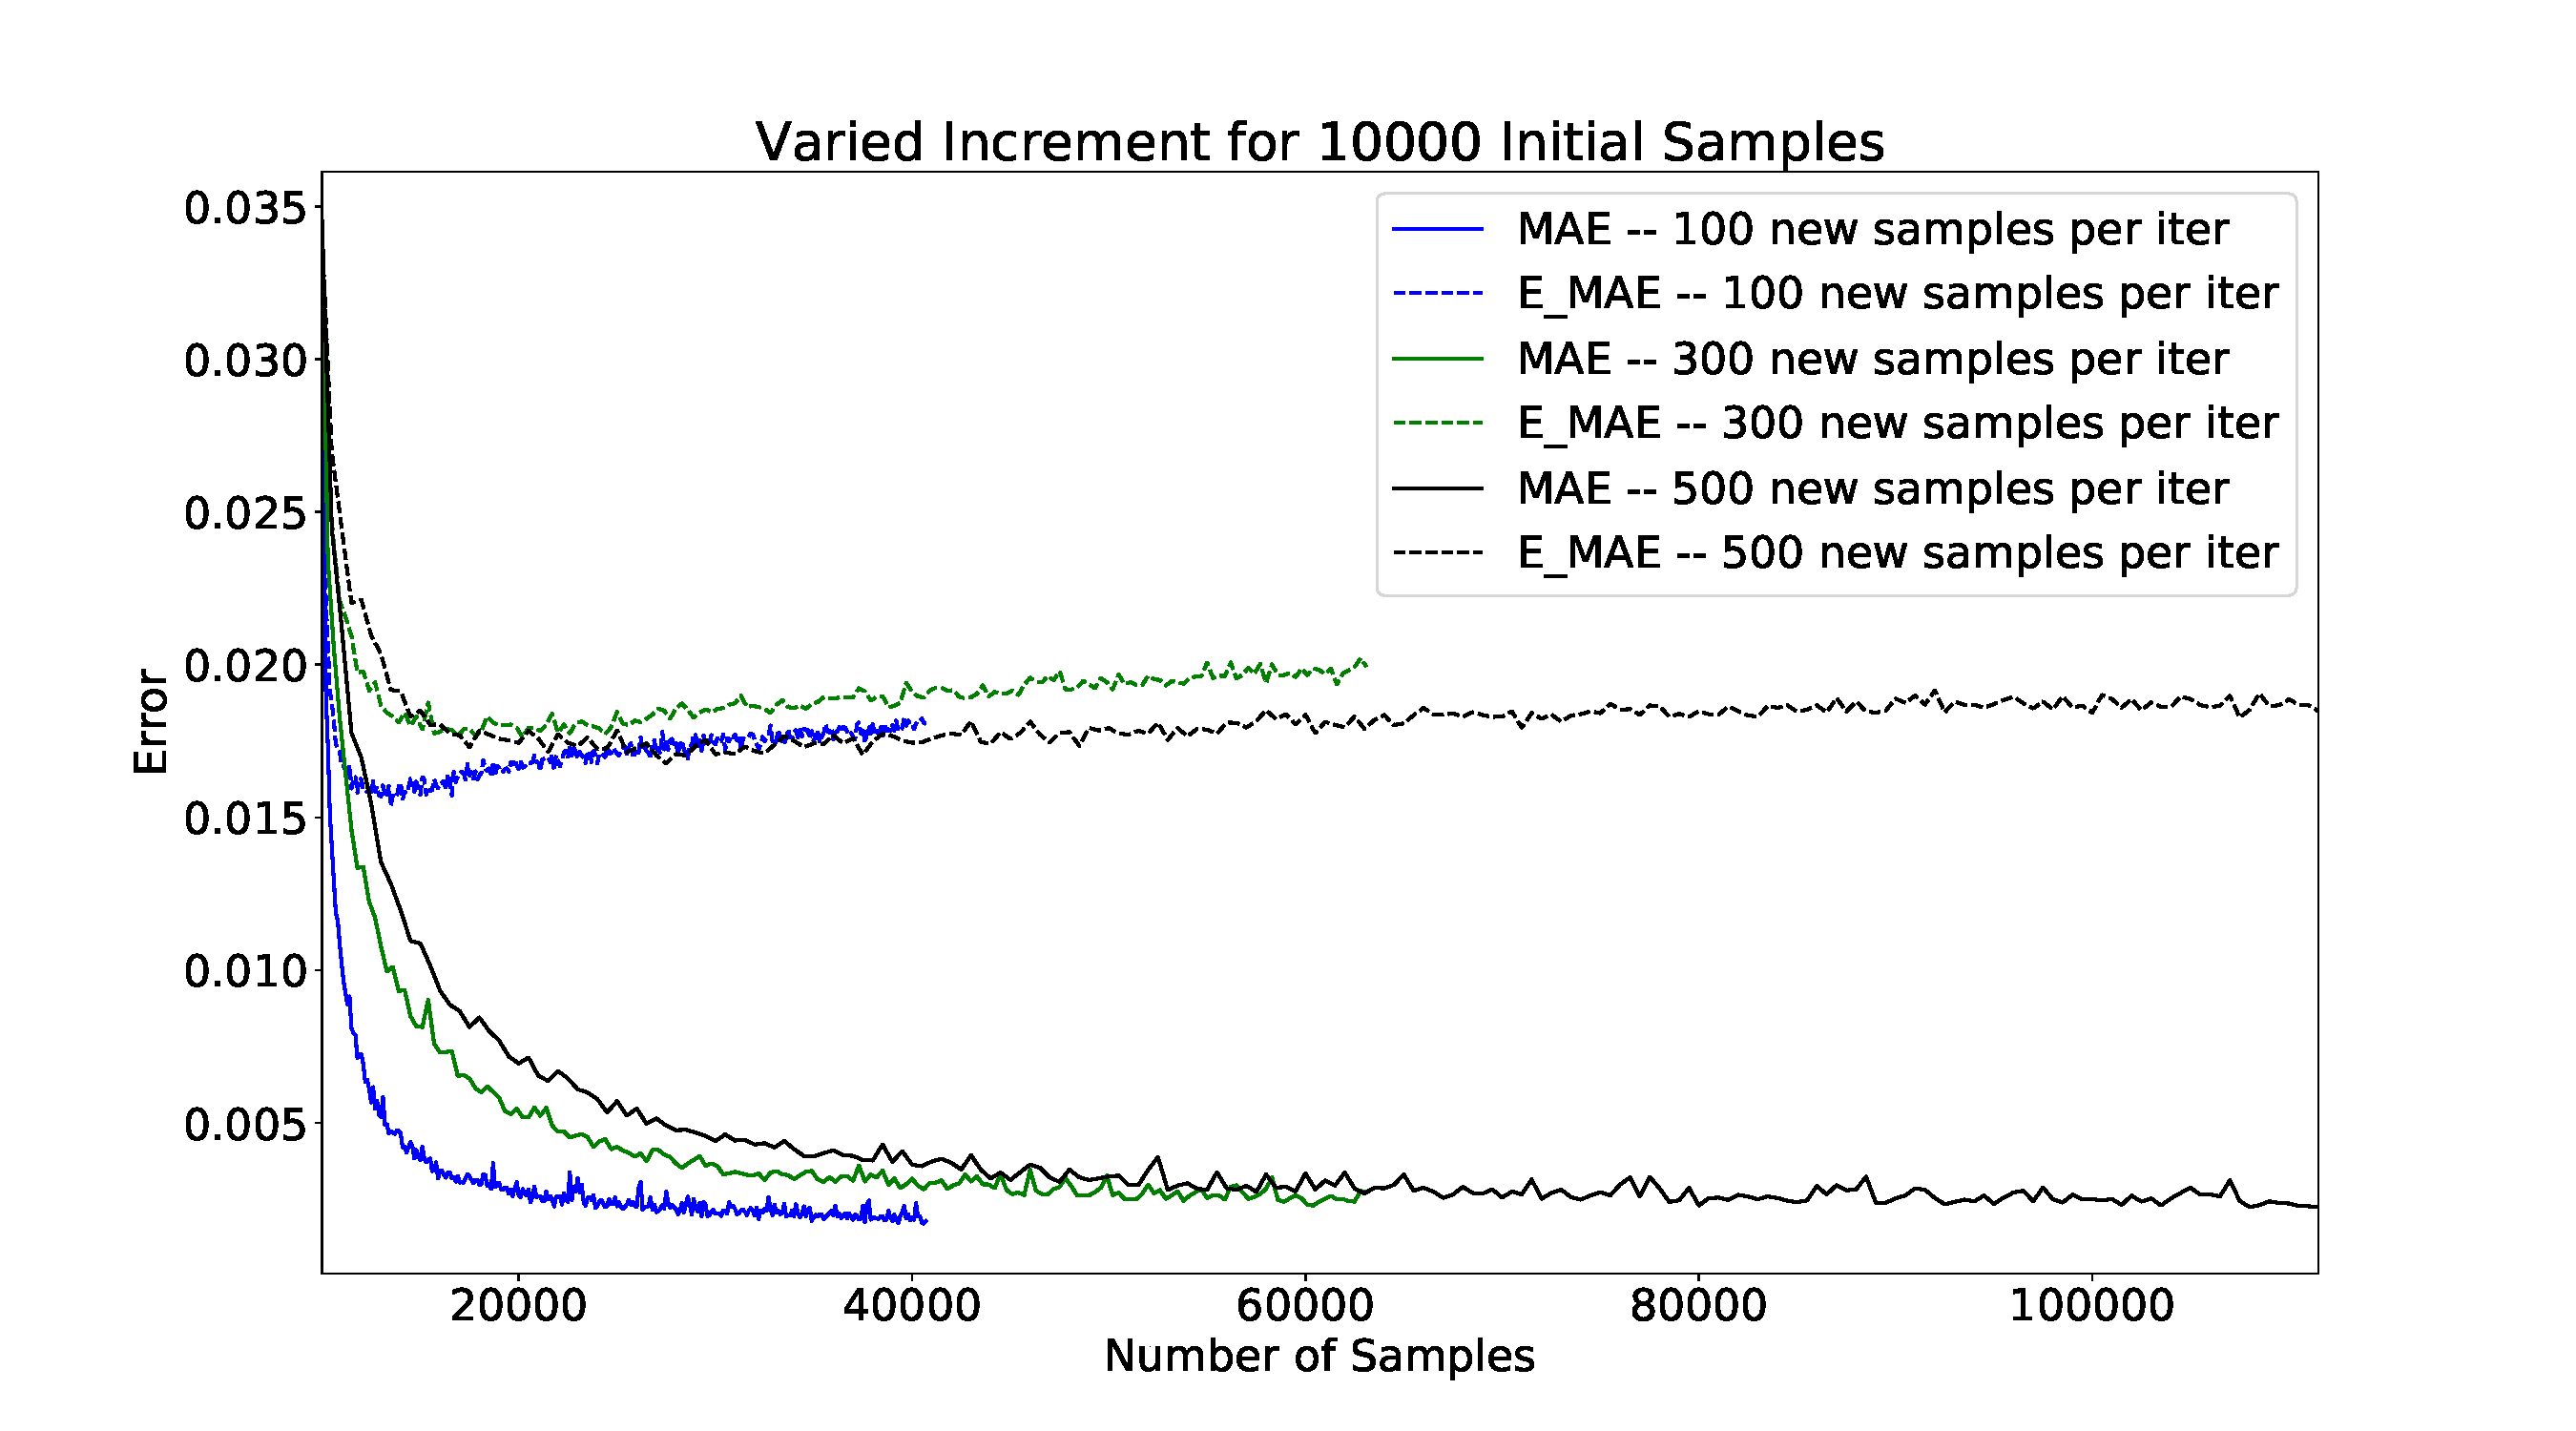
\includegraphics[width=1.1\linewidth]{fig6a_qassincrsamp.pdf}
    \end{subfigure}%
    \hfill
    \begin{subfigure}[t]{0.5\textwidth}
        \centering
        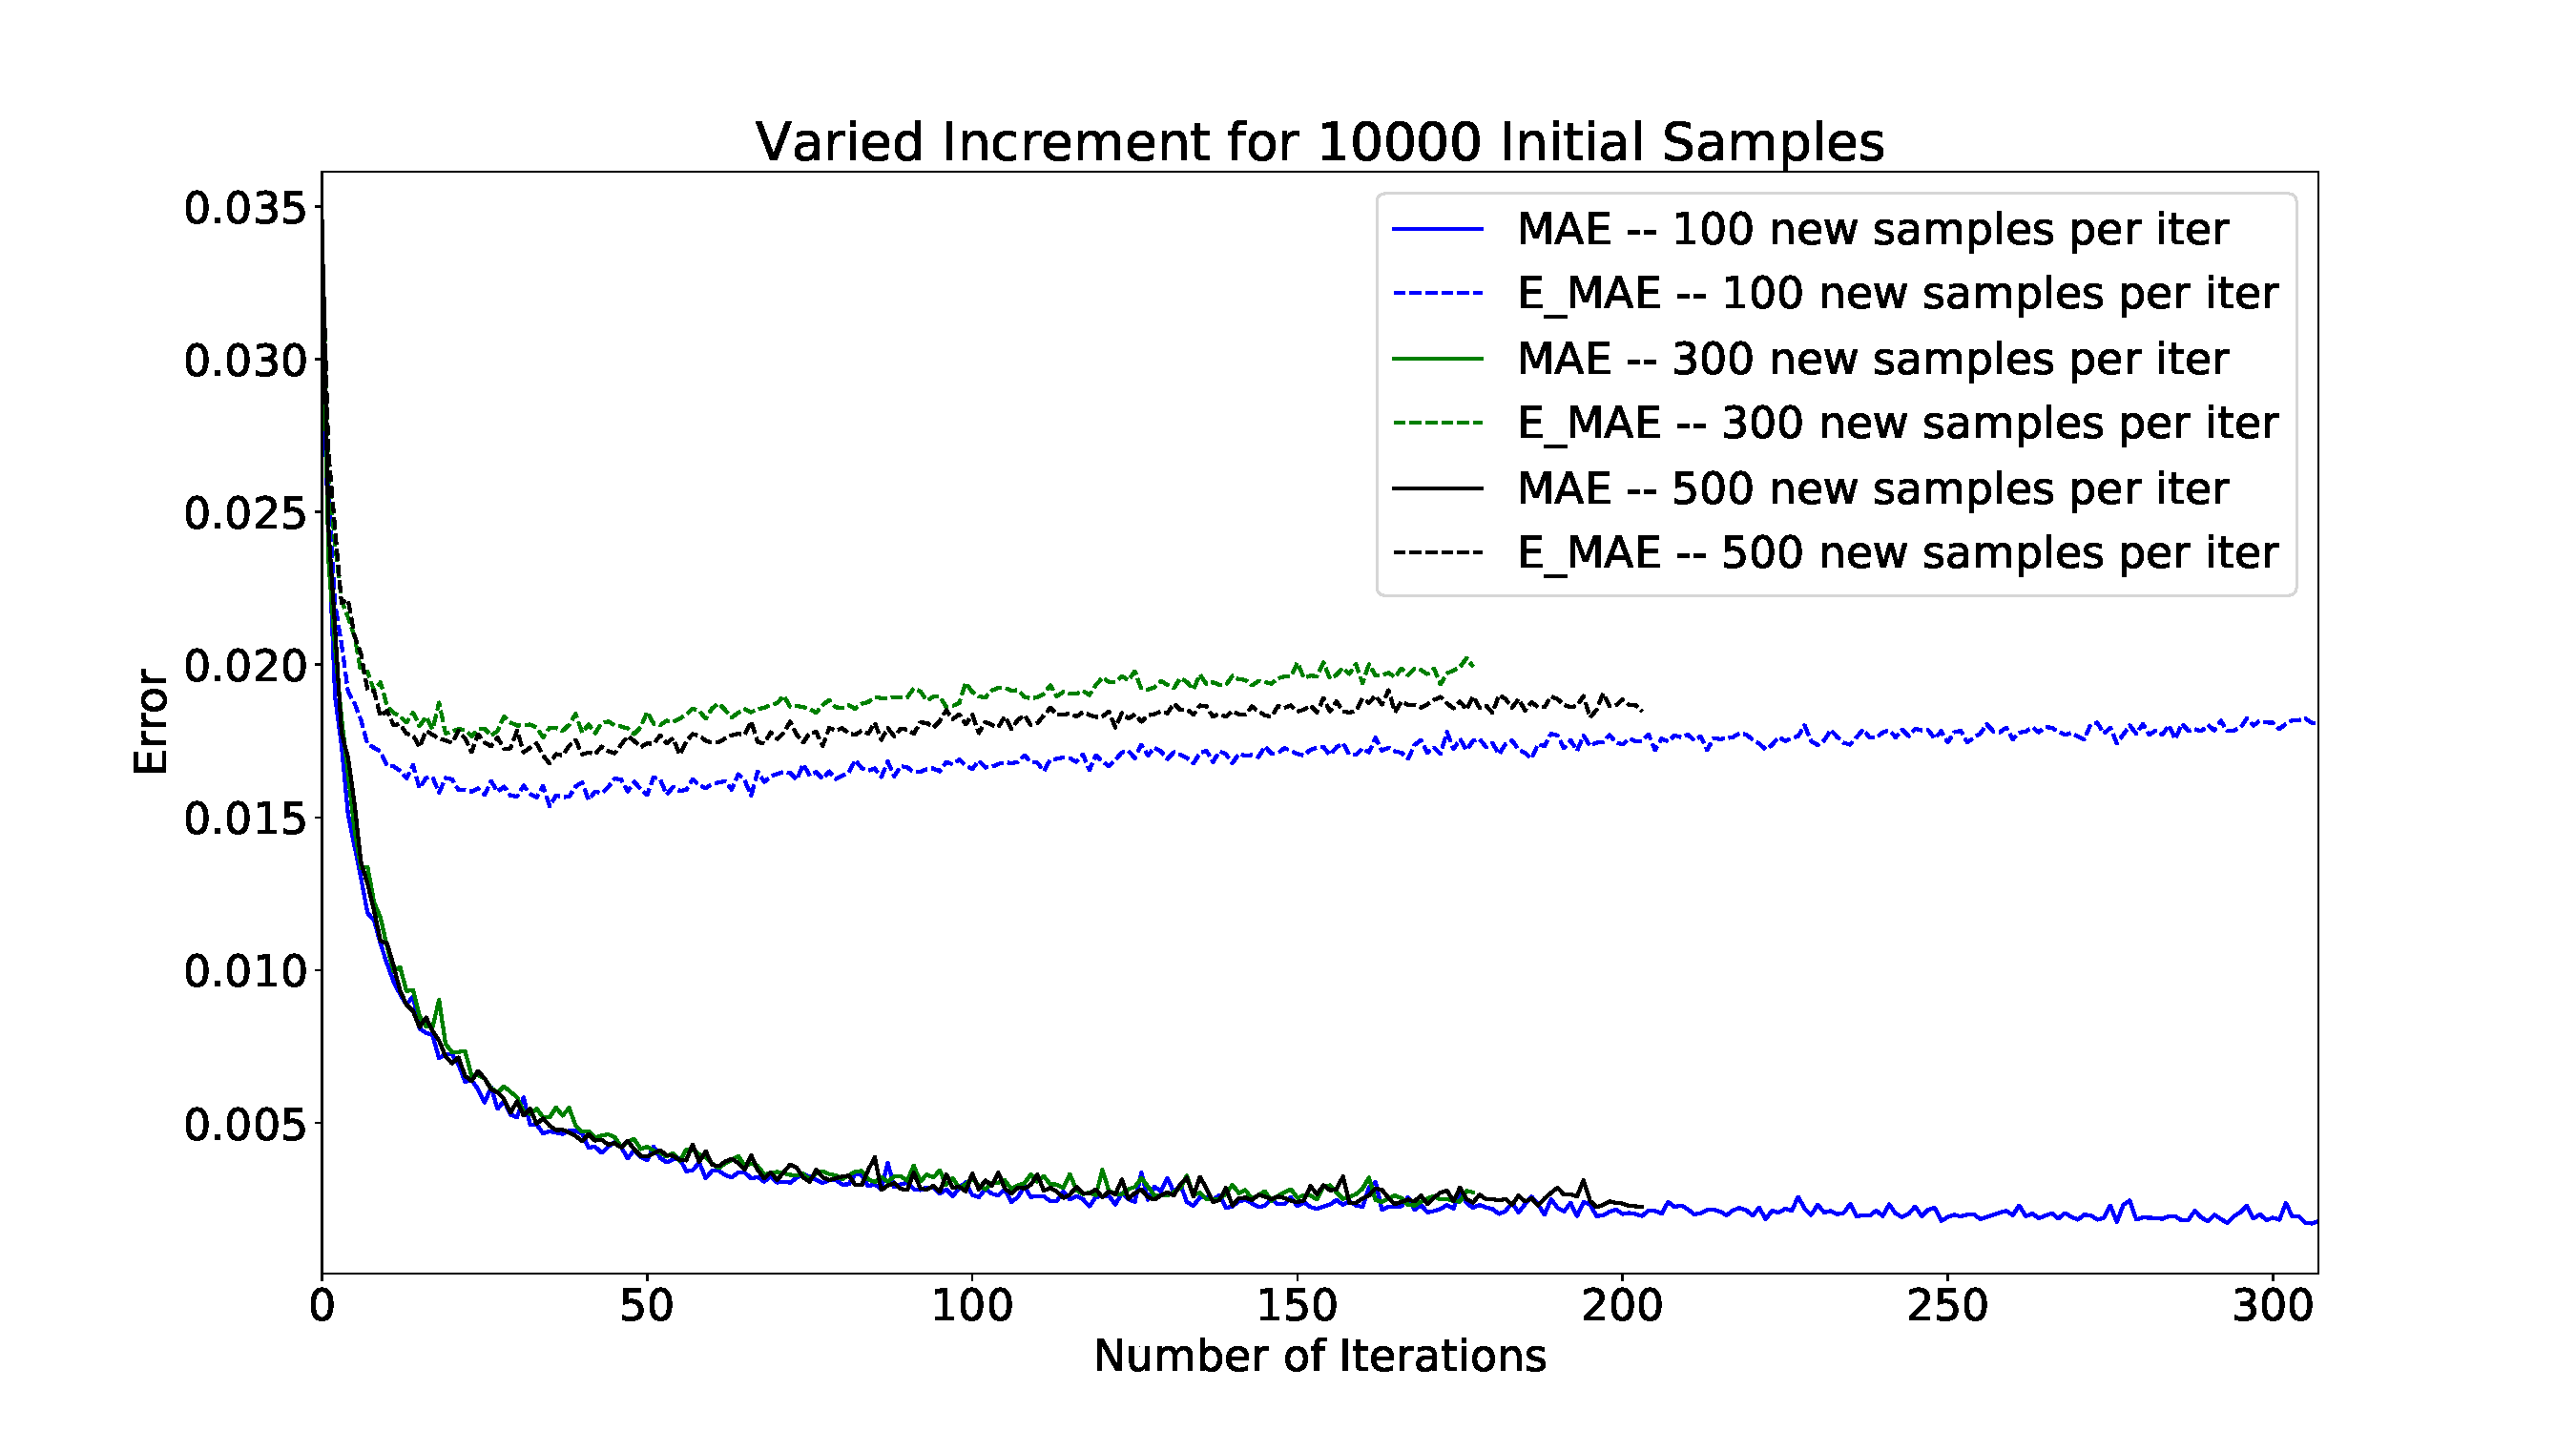
\includegraphics[width=1.1\linewidth]{fig6b_qassincrtime.pdf}
    \end{subfigure}
    \caption{QASS absolute training error over total sample quantity (left) and number of iterations (right). MAE represents surrogate error on the adaptively-sampled training/test set, and E\_MAE on the independent evaluation sets.}
    \label{fig:qassincr}
\end{figure}

The plateau effect in surrogate error on the evaluation set, seen
in~\cref{fig:qassincr}, was universal to all configurations and thought to
warrant further investigation. At first this was suspected to be a residual
effect of retraining the same ANN instance without adjustment to data
normalisation; a "Goldilocks scheme" for checking normalisation drift was
implemented and tested, but did not affect QASS performance. Schemes in which
the ANN is periodically retrained were also discarded, as the retention of
network weights from one iteration to the next was demonstrated to greatly
benefit QASS efficiency. Further insight came from direct comparison between
QASS and a baseline scheme with uniformly random incremental samples, shown
in~\cref{fig:qasssampling}.

\begin{figure}[h]
  \centering
    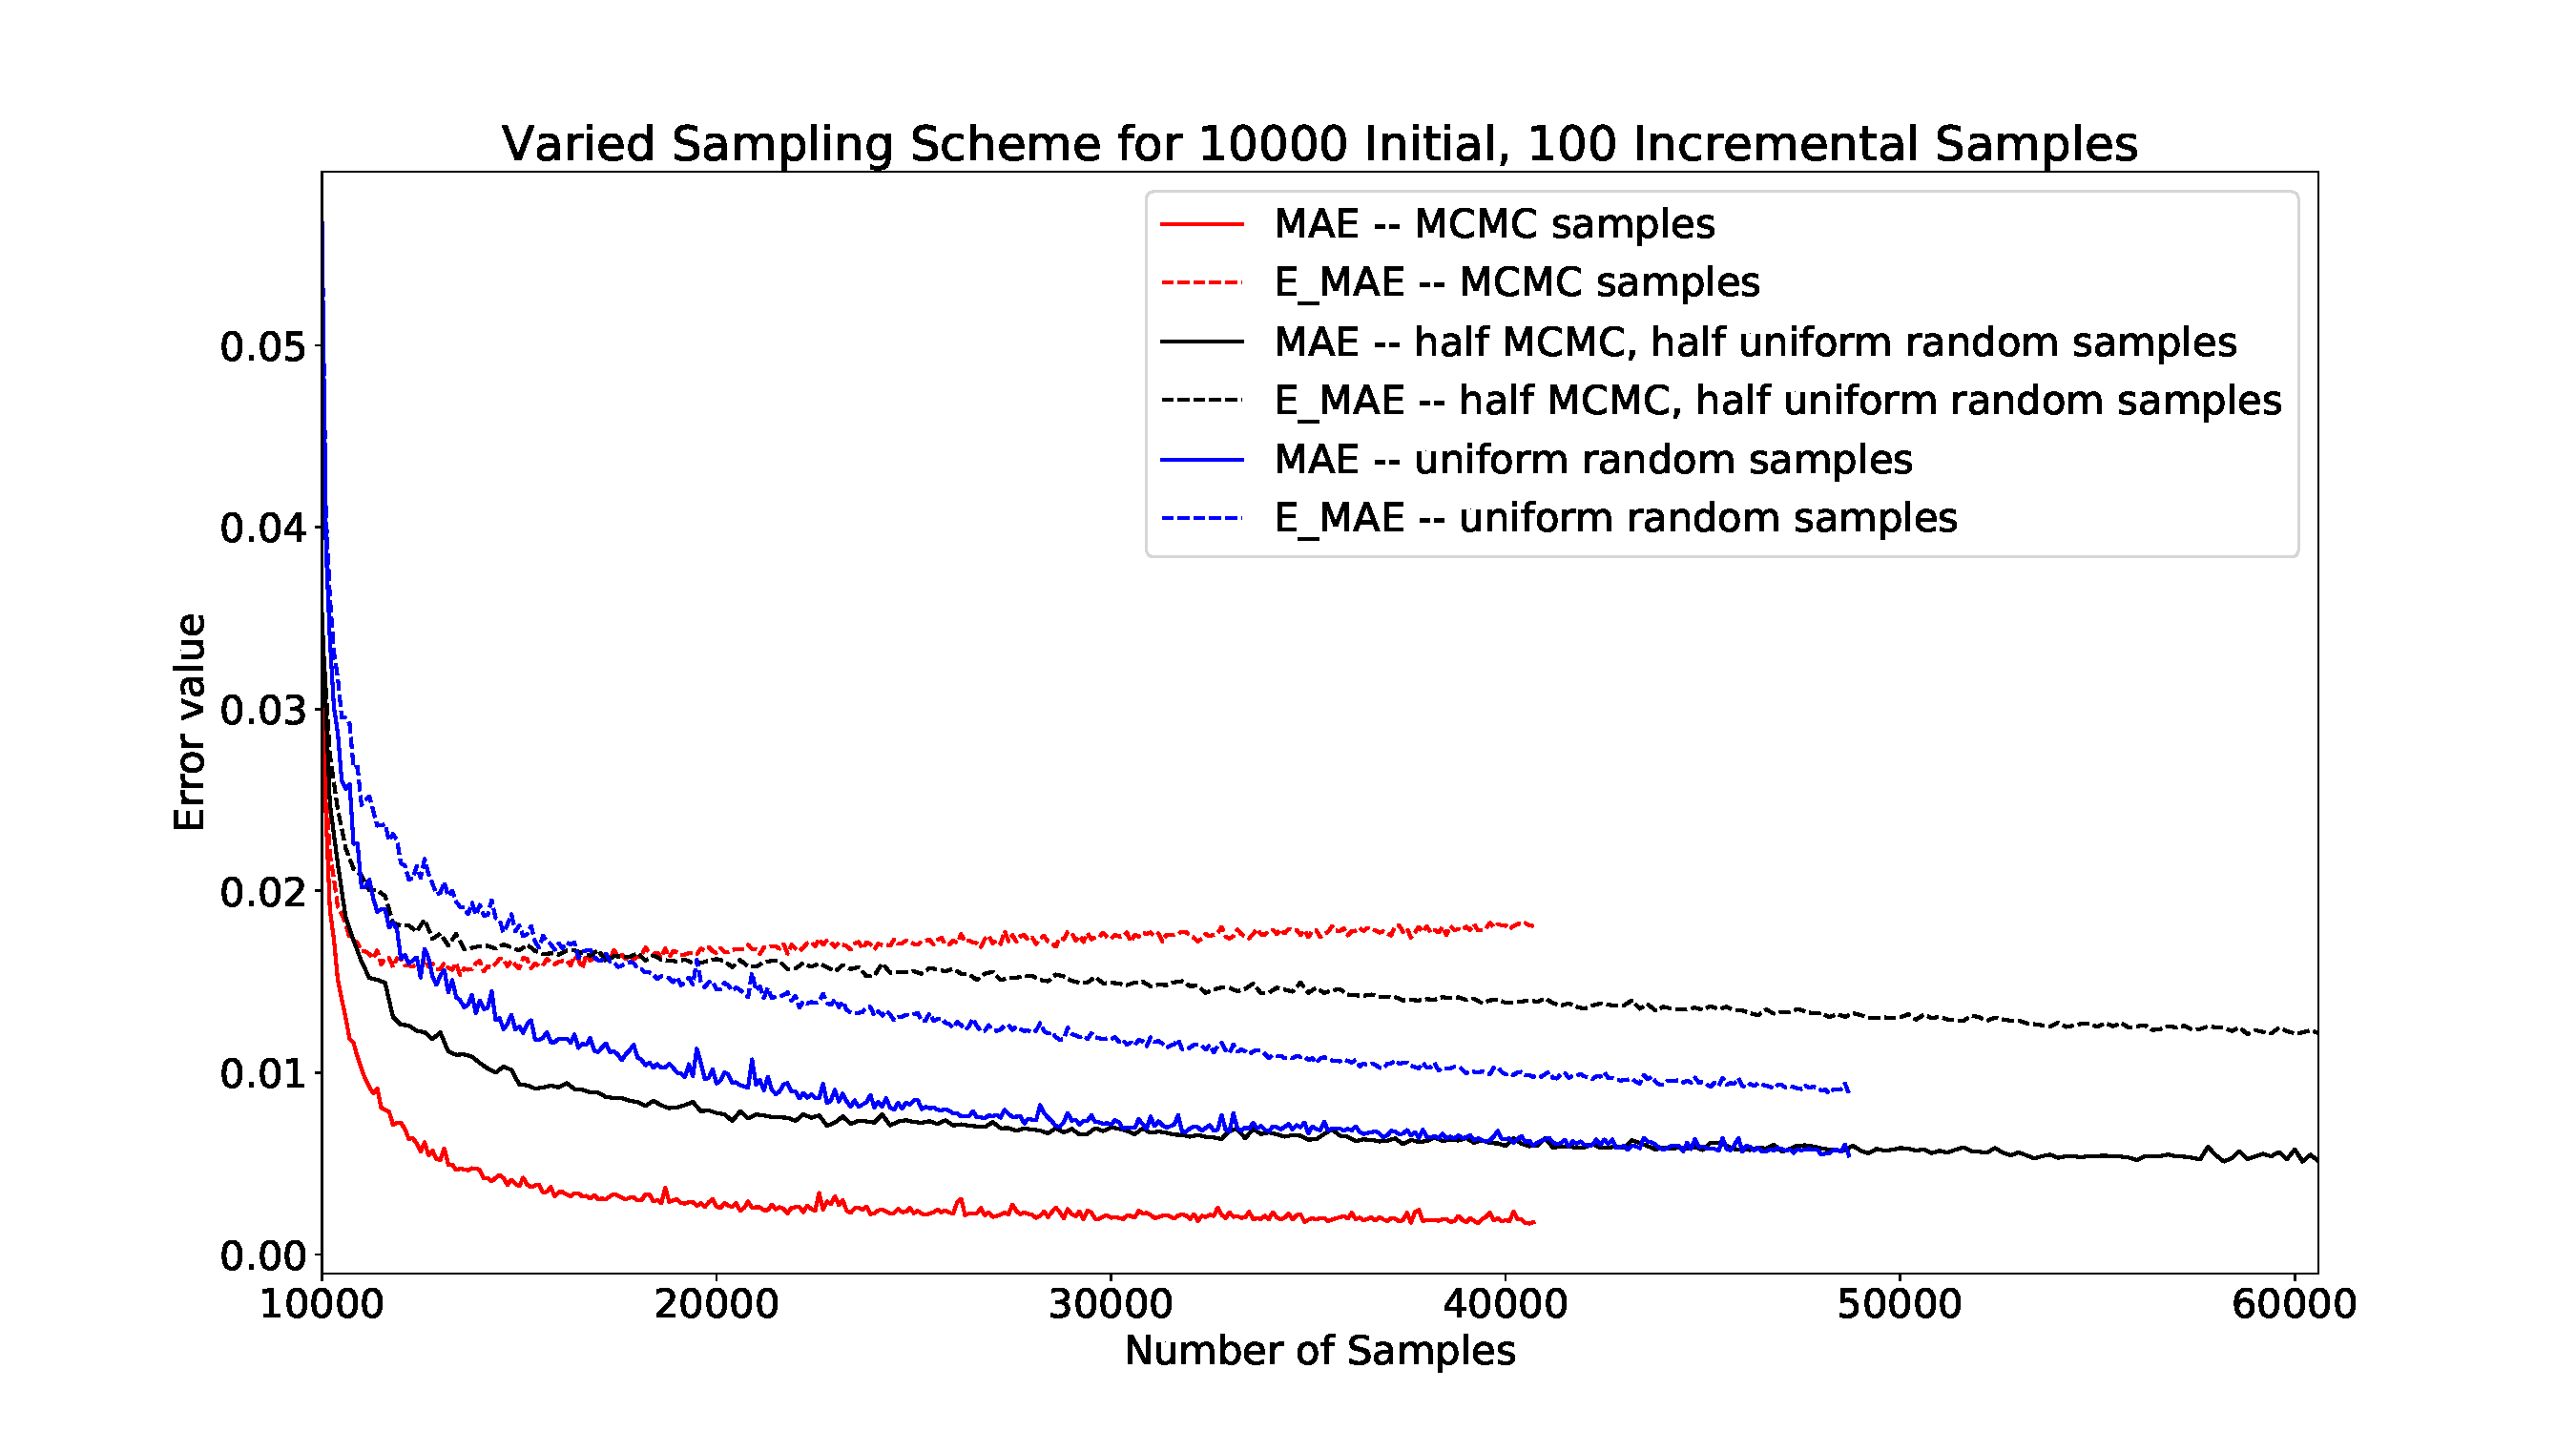
\includegraphics[width=0.78\linewidth]{fig7_qasssampling.pdf}
    \caption{Absolute training error for QASS, baseline scheme, and mixed scheme}
  \label{fig:qasssampling}
\end{figure}

Such tests revealed that while QASS has unmatched performance on its own
adaptively-sampled training set, it is outperformed by the baseline scheme on
uniformly random evaluation sets. We suspected that while QASS excels in
learning the most strongly peaked regions of the TBR theory, this comes at the
expense of precision in broader, smoother regions where uniformly random
sampling suffices. Therefore a mixed scheme was implemented, with half MCMC
samples and half uniformly random samples incremented on each iteration, which
is also shown in~\cref{fig:qasssampling}.


\section{Conclusion}
\label{sec:conclusion}
Over the course of this internship project, we employed a broad spectrum of data
analysis and machine learning techniques to develop fast and high-quality
surrogates for a~MC TBR model in use at~UKAEA. We generated over~\num{900000}
samples for training and test purposes, evaluated on this expensive MC~model. We
investigated possibilities for simplification of the parameter space, and
concluded that no straightforward reduction was possible. After reviewing
9~surrogate model families, examining their behaviour on constrained and
unrestricted feature space, and studying their scaling properties, we retrained
some of the best-performing instances to produce properties desirable for
practical use. The best approximator, trained on~\num{500000} datapoints,
featured~$R^2=\num{0.998}$ with mean prediction time
of~$\SI{0.898}{\micro\second}$, representing a relative
speedup~$\num{8659251} \times$ with respect to the MC model. Alternatively, we
also demonstrated the possibility of achieving comparable results using only a
training set of size~\num{10000}.

After a thorough review of the literature, we developed a novel adaptive
sampling algorithm, QASS, capable of interfacing with any of the individual
studied models. Preliminary testing on a toy theory, qualitatively comparable to
the MC TBR model, demonstrated the effectiveness of QASS and behavioural trends
consistent with the design of the algorithm. \textit{[Insert numerical results
for QASS.]} Further optimisation over the hyperparameter space has strong
potential to increase this performance, allowing for future deployment of QASS
on the MC TBR model in coalition with any of the most effective identified
surrogate models.


\section*{Acknowledgements}

The authors would like to thank Vignesh Gopakumar, Prof.~Nikolaos
Konstantinidis, Nikolaos Nikolaou, Prof.~Emily Nurse, Jonathan Shimwell and Ingo
Waldmann for their supervision and valuable suggestions related to this work.




%%%%%%%%%%%%%%%%%%%%%%%%%%%%%%%%%%%%%%%%%%%%%%%%%%%%%%%%%%%%%%%%%%%%%%%%%%%%%%%
% BACK MATTER
%%%%%%%%%%%%%%%%%%%%%%%%%%%%%%%%%%%%%%%%%%%%%%%%%%%%%%%%%%%%%%%%%%%%%%%%%%%%%%%

\section{Acknowledgements}
\label{sec:acknowledgements}
PM was supported the STFC UCL Centre for Doctoral Training in Data Intensive
Science (grant no. ST/P006736/1).


\section{References}
\label{sec:references}
\bibliography{ucl_tbr_paper}
\bibliographystyle{iopart-num}


\end{document}
